%% equivalence.tex - Polynomial-time kernel reductions
%%
%% Copyright 2010, 2011, 2012, 2014 Jeffrey Finkelstein.
%%
%% This LaTeX markup document is made available under the terms of the Creative
%% Commons Attribution-ShareAlike 4.0 International License,
%% https://creativecommons.org/licenses/by-sa/4.0/.
\documentclass{article}

%% This must come before hyperref.
\usepackage{amsthm}
%% These must come before hyperref.
\usepackage{thmtools}
\usepackage{thm-restate}
%% This must come before complexity.
\usepackage{hyperref}
%% This is strongly recommended by biblatex.
\usepackage[english]{babel}
%% This must come before csquotes.
\usepackage[utf8]{inputenc}
%% This is strongly recommended by biblatex.
\usepackage{csquotes}
\usepackage[backend=biber]{biblatex}
\usepackage{amsmath}
\usepackage{amssymb}
\usepackage{complexity}
\usepackage{textcomp} % for \textlangle, \textrangle
%% This is required by draftwatermark.
\usepackage{type1cm}
\usepackage[firstpage]{draftwatermark}
\usepackage{tikz}

\SetWatermarkLightness{0.9}
\SetWatermarkText{Work-in-progress}
\SetWatermarkFontSize{3.5cm}

\hypersetup{pdftitle={Polynomial time kernel reductions}, pdfauthor={Jeffrey Finkelstein}}

\addbibresource{equivalence.bib}

\declaretheorem[numberwithin=section]{theorem}
\declaretheorem[numberlike=theorem]{claim}
\declaretheorem[numberlike=theorem]{lemma}
\declaretheorem[numberlike=theorem]{proposition}
\declaretheorem[numberlike=theorem]{corollary}
\declaretheorem[numberlike=theorem, style=definition]{construction}
\declaretheorem[numberlike=theorem, style=definition]{definition}
\declaretheorem[numberlike=theorem, style=definition, name=Open problem]{openproblem}
\declaretheorem[numberlike=theorem, style=definition]{example}
\declaretheorem[numberlike=theorem, style=definition]{remark}

% create a proof sketch environment
\newenvironment{sketch}{\begin{proof}[Proof sketch]}{\end{proof}}

% custom shortcut commands
%\newcommand{\email}[1]{\href{mailto:#1}{\nolinkurl{#1}}} % formatting emails
\newcommand{\email}[1]{\textlangle\href{mailto:#1}{\nolinkurl{#1}}\textrangle}
\newcommand{\plain}[1]{\text{ #1 }} % plain text inside math environments
\newcommand{\sigmastar}{\{0, 1\}^{*}} % the set of all binary strings
\newcommand{\kj}{\overset{ker}{\oplus}} % kernel join
\newcommand{\nkr}{\nleq^{P}_{ker}} % kernel-reduces
\newcommand{\kr}{\leq^{P}_{ker}} % kernel-reduces
\newcommand{\pot}{\leq^{P}_{pot}} % potentially reduces
\newcommand{\npot}{\nleq^{P}_{pot}} % does not potentially reduce
\newcommand{\krnt}{\leq_{ker}} % kernel-reduces without time bound
\newcommand{\nkrnt}{\nleq_{ker}} % does not kernel-reduce without time bound
\newcommand{\kri}{\leq^{P}_{ker,1\text{--}1}} % 1-1 kernel-reduces
\newcommand{\mor}{\leq^{P}_{m}} % many-one reduces
\newcommand{\mornt}{\leq_m}
\newcommand{\moe}{\equiv^{P}_{m}} % many-one equivalent
\newcommand{\lb}{\left\{} % left curly brace for set notation
\newcommand{\rb}{\right\}} % right curly brace for set notation
\newcommand{\st}{\,\middle|\,} % ``such that'' pipe, for use in set definitions
\newcommand{\symdiff}{\bigtriangleup} % set symmetric difference
\newcommand{\defn}[1]{\emph{#1}} % emphasize words which are being defined
\newcommand{\pair}[2]{\left\langle#1,#2\right\rangle} % pairing function
\newcommand{\triple}[3]{\left\langle#1,#2,#3\right\rangle} % tripling function
%% \newcommand{\Q}{\textsf{Q}} % to represent an unknown quantifier
%% \newcommand{\QBF}{\lang{QBF}} % the language QBF
%% \newcommand{\QBFEq}{\lang{QBFEq}} % the language of equivalent QBFs
\newcommand{\todo}[1]{\textbf{TODO #1}}

% redefine footnote so it has no reference and no number
\long\def\symbolfootnote#1{\begingroup%
\def\thefootnote{\fnsymbol{footnote}}\footnotetext{#1}\endgroup} 

% define the author, title, and date
\author{Jeffrey~Finkelstein\\ Computer Science Department, Boston University
  \and Benjamin~Hescott\\ Computer Science Department, Tufts University}
\title{Polynomial time kernel reductions}

\begin{document}

\maketitle

%% abstract.tex - a brief summary of the work
%%
%% Copyright 2010, 2011, 2012, 2014, 2015 Jeffrey Finkelstein.
%%
%% This LaTeX markup document is made available under the terms of the Creative
%% Commons Attribution-ShareAlike 4.0 International License,
%% https://creativecommons.org/licenses/by-sa/4.0/.
\begin{abstract}
  In the framework of computational complexity, and in an effort to define a more natural reduction for problems of equivalence, we investigate the recently introduced \emph{kernel reduction}, a reduction that operates on each element of a pair independently.
  %% This reduction, defined only on equivalence problems, differs from the usual many-one reduction in that it transforms each string in a pair independently; for example, a kernel reduction from undirected to directed graph isomorphism is a function from undirected to directed graphs whereas a many-one reduction is a function from pairs of undirected graphs to pairs of directed graphs.
  This paper details the limitations and uses of kernel reductions.
  % Summary
  %
  % findings (focus on author) what? - what the work revealed when performing the task
  We show that kernel reductions are weaker than many-one reductions and provide conditions under which complete problems exist.
  % We prove that for polynomial time, kernel reductions are strictly weaker than many-one reductions.
  % We also provide sufficient conditions for completeness under kernel reductions, show the relationship between kernel and many-one completeness, and prove the existence of equivalence problems under intermediate difficulty under a standard assumption.
  % conclusion (focus on readers) so what? - what the findings mean for the audience
  Ultimately, the number and size of equivalence classes can dictate the existence of a kernel reduction. %%, regardless of the complexity of the equivalence problem.
  % perspective (focus on anyone) what now? - what should be done next
  We leave unsolved the unconditional existence of a complete problem under polynomial-time kernel reductions for the standard complexity classes.
  %% The most important open problem we leave unsolved is proving the unconditional existence of a complete problem under kernel reductions for some basic complexity classes that are well-known to have complete problems under many-one reductions.
\end{abstract}

%% copyright.tex - the copyright notice for this paper
%%
%% Copyright 2010, 2011, 2012, 2014, 2015 Jeffrey Finkelstein.
%%
%% This LaTeX markup document is made available under the terms of the Creative
%% Commons Attribution-ShareAlike 4.0 International License,
%% https://creativecommons.org/licenses/by-sa/4.0/.
\symbolfootnote{%
  Copyright 2010, 2011, 2012, 2014, 2015 Jeffrey~Finkelstein and Benjamin~Hescott.

  This document is licensed under the Creative Commons Attribution-ShareAlike 4.0 International License, which is available at \mbox{\url{https://creativecommons.org/licenses/by-sa/4.0/}}.
  The \LaTeX{} markup that generated this document can be downloaded from its website at \mbox{\url{https://github.com/jfinkels/equivalence}}.
  The markup is distributed under the same license.
}


%% introduction.tex - introduction and motivation for the work
%%
%% Copyright 2010, 2011, 2012, 2014, 2015 Jeffrey Finkelstein.
%%
%% This LaTeX markup document is made available under the terms of the Creative
%% Commons Attribution-ShareAlike 4.0 International License,
%% https://creativecommons.org/licenses/by-sa/4.0/.
\section{Introduction}
% Foreword

% context (focus on anyone) why now? - current situation, and why the need is so important
Determining the computational complexity of deciding whether two graphs are isomorphic has significant implications in nearly every field of computer science.
One main technique for determining the complexity of the problem is showing how the difficulty of the problem relates to the difficulty of other known problems.
The relative difficulty of computational problems are often compared using the many-one reduction, a function by which we encode an instance of a problem as an instance of another problem.
In the case of the graph isomorphism problem, a many-one reduction from the graph isomorphism problem to, for example, the directed graph isomorphism problem allows the function computing the reduction to have access to both graphs in an instance of the problem.
However, access to both graphs is not necessary for computing the reduction; the function transforms each undirected graph independently into a directed graph.
In other words, the reduction is in reality defined on the domain of graphs, not on the domain of pairs of graphs.
This is a far more natural way to define reductions between problems of equivalence, and is furthermore a finer-grained comparison of the relative difficulty of the two computational problems.

% need (focus on readers) why you? - why this is relevant to the reader, and why something needed to be done
The \emph{kernel reduction}, defined in \autocite[Definition~4.13]{fg11}, formally captures this notion of reduction among computational problems of equivalence involving independent transformation of each element of a pair.
This type of reduction has appeared previously under other names not only in this setting but also in more general settings (``Borel reduction''\kern-0.5em, ``strong isomorphism reduction''\kern-0.5em, ``strong equivalence reduction''\kern-0.5em, ``relation reduction''\kern-0.5em, ``component-wise reduction''\kern-0.5em, etc.).
To the best of our knowledge, every known many-one reduction between problems of equivalence is really a kernel reduction (see, for an early example, the list of problems many-one reducible to graph isomorphism given in \autocite{bc79}).
Since most reductions between problems of equivalence seem to be kernel reductions, are they truly useful in theory or in practice?
If so, since the kernel reduction has access only to one element of a pair at a time, what are the limitations of kernel reductions?

%%% relevant existing work, given as part of the need
Some of our theorems adapt or clarify existing work in order to have simpler, self-contained, complexity-theoretic proofs of important theorems about kernel reductions.
In \autocite{fg11}, the authors ask whether kernel reductions and many-one reductions are provably different.
However, little beyond the definition is given there, other than the general idea that an imbalance in the number of equivalence classes of the two equivalence problems prevents the existence of a kernel reduction.
In computability theory, a similar type of reduction between equivalence problems has been well-studied by a series of recent papers (for example, \autocite{gg01, ff12, ffn12, chm12, imnn13, almnss14, mn14}).
However, these papers do not focus on efficiently computable reductions.
In \autocite{bcffm}, the authors provide a thorough treatment of not only the kernel reduction but also a generalization called the ``strong isomorphism reduction''\kern-0.5em.
%% We modify some of their techniques to prove theorems, some more general and some more specific than in that work, in a way that requires only some basic knowledge of complexity theory.
The authors of \autocite{gz14} extended the work of \autocite{bcffm}, and in doing so, independently proved the main combinatorial idea used in this paper to examine the limitations of kernel reductions.
This paper, complementing that work, focuses mainly on completeness results.

% task (focus on author) why me? - what was undertaken to address the need
We undertake a thorough investigation of the basic properties of kernel reductions, comparing them with the basic properties of many-one reductions.
% object (focus on document) why this document - what the document covers
The starting point for understanding many-one reductions is $\P$ and $\NP$, so we attempt to extend the definition from \autocite{fg11} of $\PEq$, the class of equivalence problems decidable in polynomial time, to the definition of the complexity class $\NPEq$ (\autoref{sec:definitions}).
We determine the limitations of kernel reductions; these appear to be combinatorial, not computational, in nature (\autoref{sec:limitations}).
We discover sufficient conditions for complete problems under kernel reductions in classes of equivalence problems (\autoref{sec:generalcompleteness}).
We compare the new notion of completeness under kernel reductions with the usual notion of completeness under many-one reductions (\autoref{sec:npeqcompleteness}).
Finally, as an analog to $\NP$-intermediary problems with respect to many-one reductions, we examine the possibility of $\NPEq$-intermediary problems with respect to kernel reductions (\autoref{sec:intermediary}).

%%%%
%% preliminaries.tex
%%
%% Copyright 2011, 2012 Jeffrey Finkelstein
%%
%% Except where otherwise noted, this work is made available under the terms of
%% the Creative Commons Attribution-ShareAlike 3.0 license,
%% http://creativecommons.org/licenses/by-sa/3.0/.
%%
%% You are free:
%%    * to Share — to copy, distribute and transmit the work
%%    * to Remix — to adapt the work
%% Under the following conditions:
%%    * Attribution — You must attribute the work in the manner specified by
%%    the author or licensor (but not in any way that suggests that they
%%    endorse you or your use of the work).
%%    * Share Alike — If you alter, transform, or build upon this work, you may
%%    distribute the resulting work only under the same, similar or a 
%%    compatible license.
%%    * For any reuse or distribution, you must make clear to others the 
%%    license terms of this work. The best way to do this is with a link to the
%%    web page http://creativecommons.org/licenses/by-sa/3.0/.
%%    * Any of the above conditions can be waived if you get permission from
%%    the copyright holder.
%%    * Nothing in this license impairs or restricts the author's moral rights.
%%%%
\section{Preliminaries}
\label{sec:preliminaries}

If $f\colon S\to T$ is a well-defined function and $S'\subseteq S$, then \defn{$f$ restricted to the domain $S'$} is the function $f'\colon S'\to T$ defined by $f'(x)=f(x)$ for all $x\in S'$.
We denote this restricted function on a smaller domain by $f|_{S'}$.

If $\Sigma$ is an alphabet then $\Sigma^*$ is the set of all strings over the alphabet $\Sigma$ and $\Sigma^{\leq n}$ is the set $\lb w\in\Sigma^* \st |w|\leq n \rb$.
Usually $\Sigma$ is the binary alphabet $\{0, 1\}$.
The empty string will be denoted by $\lambda$.
If $\sigma\in\Sigma$ then $\sigma^k$ is the string consisting of $k$ concatenated copies of the symbol $\sigma$.
If $x$ and $y$ are elements of $\Sigma^*$, then we denote by $\pair{x}{y}$ the \defn{pairwise encoding} of $x$ and $y$, which is itself an element of $\Sigma^*$.
In this paper, we will assume the reasonable pairwise encoding defined by $\pair{x}{y}=x_1x_1x_2x_2\cdots x_{|x|}x_{|x|}01y_1y_1y_2y_2\cdots y_{|y|}y_{|y|}$ for all $x$ and $y$ in $\Sigma^*$.
As usual, a \defn{language} over an alphabet $\Sigma$ is a subset of $\Sigma^*$.
The \defn{complement} of a language $L$ is $\Sigma^*\backslash L$, and is denoted $\overline{L}$.

The complexity classes $\P$, $\NP$, $\FP$ (polynomial time computable functions), $\SKP$, $\PKP$, and $\PSPACE$ have the usual definitions.
The set of words accepted by a Turing machine $M$ is denoted $L(M)$.
The \defn{complement} of a complexity class $\mathcal{C}$ is the set of complements of languages in $\mathcal{C}$, and is denoted $\coC$.

We say a Turing machine $M$ is a \defn{polynomially clocked Turing machine} if the description of $M$ includes a positive integer $k$ such that $M$ halts within time $kn^k$ on all inputs of length $n$.

If $L_1, L_2$ are languages, we say that \defn{$L_1$ polynomial time many-one reduces to $L_2$} if there exists a polynomial time computable function $f$ such that $w\in L_1$ if and only if $f(w)\in L_2$.
We denote this by $L_1\mor L_2$.
If $L_1\mor L_2$ and $L_2\mor L_1$, we say that $L_1$ and $L_2$ are \defn{equivalent under polynomial time many-one reductions}, and denote this by $L_1\moe L_2$.

Given a universe $U$, $R\subseteq U\times U$ is an \defn{equivalence relation on $U$} if $R$ is
\begin{enumerate}
\item reflexive: for all $x\in U$, $(x,x)\in R$
\item symmetric: for all $x,y\in U$, $(x,y)\in R$ implies $(y,x)\in R$
\item transitive: for all $x,y,z\in U$, $(x,y)\in R$ and $(y,z)\in R$ implies $(x,z)\in R$
\end{enumerate}
An equivalence relation $R$ can be encoded as a language by taking the pairwise encoding of each pair in $R$.
In this way we can study the computational complexity of classes of languages which represent equivalence relations.
In this paper we will abuse notation and write $\pair{x}{y}\in R$ for an equivalence relation $R$ on $\Sigma^*$, but what we really mean is $(x,y)\in R$ and $\pair{x}{y}\in L_R$, the language on the alphabet $\Sigma$ induced by $R$.

The \defn{equivalence class} of $x$ with respect to an equivalence relation $R$ on $U$ is $\lb y\in U \st (x,y)\in R \rb$. It is denoted $[x]_R$, or if the context is clear, simply $[x]$.
Each element $x\in U$ is in exactly one equivalence class, so the equivalence classes of an equivalence relation on $U$ provide a partition of $U$.

A \defn{complete invariant} for an equivalence relation $R$ on $U$ is a function $f\colon U\to T$ such that for all $x,y\in U$, $(x,y)\in R$ if and only if $f(x)=f(y)$.
In \autoref{sec:definitions} we will define generalizations of the complete invariant which accept as input an additional witness to the equivalence of $x$ and $y$.

\defn{$\PEq$} is the class of equivalence relations for which membership can be decided by a Turing machine running in deterministic polynomial time.
\defn{$\NPEq$} is the class of equivalence relations for which membership can be decided by a Turing machine running in non-deterministic polynomial time.
In other words, $\PEq$ is the set of (languages induced by) equivalence relations which are in \P, and $\NPEq$ is the set of (languages induced by) equivalence relations which are in \NP.
In general, the class \defn{$\CEq$} is the class of languages induced by equivalence relations which are in the complexity class $\mathcal{C}$.
As usual, $\PEq\subseteq\NPEq$.
%\defn{$\Ker$} is the class of equivalence relations which have a polynomial time computable complete invariant.

We now require a natural notion of reduction among equivalence relations.
If $R$ and $S$ are equivalence relations on $\Sigma^*$, we say $R$ \defn{kernel reduces to} $S$ if there exists a computable $f\colon\Sigma^*\to\Sigma^*$ such that $\forall x,y\in\Sigma^*$, $\pair{x}{y}\in R\iff \pair{f(x)}{f(y)}\in S$.
We denote this by $R\krnt S$.
If $f$ is computable in polynomial time, then we say $R$ \defn{polynomial time kernel reduces to} $S$ and use the notation $R\kr S$.

Notice the difference between a kernel reduction and a regular old many-one reduction: a kernel reduction maps $\pair{x}{y}\in R$ to $\pair{f(x)}{f(y)}\in S$, whereas a many-one reduction maps $\pair{x}{y}\in R$ to $f(\pair{x}{y})\in S$, for some polynomial time computable function $f$.
Informally, a function which computes a many-one reduction has access to both $x$ and $y$ but a function which computes a kernel reduction has access to only one of $x$ and $y$ at a time.
Note that since it is more restrictive, a kernel reduction induces a many-one reduction (namely the function $\pair{x}{y}\mapsto\pair{f(x)}{f(y)}$).

As an analog to polynomial time many-one completeness in \NP, we define a similar notion of completeness under polynomial time kernel reductions in \NPEq.
An equivalence relation $S$ is \defn{\NPEq-hard} if for all $R\in\NPEq$, $R\kr S$.
If $S$ is also in \NPEq, then it is \defn{\NPEq-complete}.
If $S$ is \NPEq-complete, we sometimes say that $S$ is \defn{complete under $\kr$ reductions in \NPEq}.
Generally, an equivalence relation $S$ is \defn{$\CEq$-hard} if for all $R\in\CEq$, $R\kr S$, and \defn{$\CEq$-complete} if it is additionally in $\CEq$.

%%%%
%% definitions.tex
%%
%% Copyright 2011, 2012 Jeffrey Finkelstein
%%
%% Except where otherwise noted, this work is made available under the terms of
%% the Creative Commons Attribution-ShareAlike 3.0 license,
%% http://creativecommons.org/licenses/by-sa/3.0/.
%%
%% You are free:
%%    * to Share — to copy, distribute and transmit the work
%%    * to Remix — to adapt the work
%% Under the following conditions:
%%    * Attribution — You must attribute the work in the manner specified by
%%    the author or licensor (but not in any way that suggests that they
%%    endorse you or your use of the work).
%%    * Share Alike — If you alter, transform, or build upon this work, you may
%%    distribute the resulting work only under the same, similar or a 
%%    compatible license.
%%    * For any reuse or distribution, you must make clear to others the 
%%    license terms of this work. The best way to do this is with a link to the
%%    web page http://creativecommons.org/licenses/by-sa/3.0/.
%%    * Any of the above conditions can be waived if you get permission from
%%    the copyright holder.
%%    * Nothing in this license impairs or restricts the author's moral rights.
%%%%
\section{Definitions of \texorpdfstring{\NPEq}{NPEq}}
\label{sec:definitions}

In this section we examine possible alternate definitions of \NPEq.
The main property of languages in $\NP$ is that membership in each language is verifiable in polynomial time, given a witness to the membership.
We propose here several possible definitions of $\NPEq$ in order to determine which make sense, which are too restrictive, and which are equivalent.

For the sake of brevity, in all definitions below, when we write $\exists w$, we mean $\exists w$ with length polynomially bounded with respect to the length of $x$, $y$, or the pair $\pair{x}{y}$ (depending on the requirements of the particular definition).

The first two definitions are analogs of the two fundamental definitions of \NP.
\begin{definition}\label{def:npeq1}
  An equivalence relation $R$ is in $\NPEqOne$ if there exists a non-deterministic Turing machine, call it $N$, which halts in time polynomial in the length of the input, such that
  \begin{displaymath}
    \pair{x}{y}\in R\iff N(\pair{x}{y})\plain{accepts}
  \end{displaymath}
\end{definition}
\begin{definition}\label{def:npeq2}
  An equivalence relation $R$ is in $\NPEqTwo$ if there exists a language $L\in\P$ such that
  \begin{displaymath}
    \pair{x}{y}\in R\iff \exists w\colon \pair{\pair{x}{y}}{w}\in L
  \end{displaymath}
\end{definition}

The next two definitions attempt to require that the witness language is itself an equivalence relation, instead of an arbitrary language in $\P$, as in \autoref{def:npeq2}.
\begin{definition}\label{def:npeq3}
  An equivalence relation $R$ is in $\NPEqThree$ if there exists an equivalence relation $R'\in \PEq$ such that
  \begin{displaymath}
    \pair{x}{y}\in R\iff \exists w_x,w_y\colon \pair{\pair{x}{w_x}}{\pair{y}{w_y}}\in R'
  \end{displaymath}
\end{definition}
\begin{definition}\label{def:npeq4}
  An equivalence relation $R$ is in $\NPEqFour$ if there exists an equivalence relation $R'\in \PEq$ such that
  \begin{displaymath}
    \pair{x}{y}\in R\iff \exists w\colon \pair{\pair{x}{w}}{\pair{y}{w}}\in R'
  \end{displaymath}
\end{definition}

The next two definitions attempt to allow the possibility of not just a simple string which witnesses the equivalence of $x$ and $y$, but a ``witness function'' which may map $x$ and $y$, along with witness strings, to an equivalence relation in \PEq.
\begin{definition}\label{def:npeq5}
  An equivalence relation $R$ is in $\NPEqFive$ if there exists an equivalence relation $R'\in \PEq$ and a function $f\in\FP$ such that
  \begin{displaymath}
    \pair{x}{y}\in R\iff \exists w_x,w_y\colon \pair{f(x, w_x)}{f(y, w_y)}\in R'
  \end{displaymath}
\end{definition}
\begin{definition}\label{def:npeq6}
  An equivalence relation $R$ is in $\NPEqSix$ if there exists an equivalence relation $R'\in \PEq$ and a function $f\in\FP$ such that
  \begin{displaymath}
    \pair{x}{y}\in R\iff \exists w\colon \pair{f(x, w)}{f(y, w)}\in R'
  \end{displaymath}
\end{definition}

The final two definitions attempt to describe equivalence relations for which there is a ``witnessed complete invariant'', which maps equivalent strings to equal strings when given access to some witness of their equivalence.
We say that an equivalence relation $R$ on a universe $U$ has a \defn{one-witness complete invariant} if there exists a function $f\colon U\times S\to T$ such that $(x,y)\in R$ if and only if $\exists w\in S\colon f(x, w)=f(y, w)$, and we say that it has a \defn{two-witness complete invariant} if $(x, y)\in R$ if and only if $\exists w_x, w_y\in S\colon f(x, w_x)=f(y, w_y)$.
\begin{definition}\label{def:npeq7}
  An equivalence relation $R$ is in $\NPEqSeven$ if it has a polynomial time computable two-witness complete invariant, that is, a function $f\in\FP$ such that
  \begin{displaymath}
    \pair{x}{y}\in R\iff \exists w_x, w_y\colon f(x, w_x) = f(y, w_y)
  \end{displaymath}
\end{definition}
\begin{definition}\label{def:npeq8}
  An equivalence relation $R$ is in $\NPEqEight$ if it has a polynomial time computable one-witness complete invariant, that is, a function $f\in\FP$ such that
  \begin{displaymath}
    \pair{x}{y}\in R\iff \exists w\colon f(x, w) = f(y, w)
  \end{displaymath}
\end{definition}

\autoref{fig:inclusions} shows the inclusions among each of the classes of equivalence relations defined above.
\begin{figure}
  \caption{\label{fig:inclusions}Inclusions among possible definitions of equivalence relations verifiable in deterministic polynomial time.}
  \begin{displaymath}
    \xymatrix{%
      \NPEqSeven \ar[r] & \NPEqFive \ar[r] & \NPEqThree \ar[r] & \NPEqTwo \ar@{<->}[r] & \NPEqOne \\
      \NPEqEight \ar[u] \ar[r] & \NPEqSix \ar[u] \ar[r] & \NPEqFour \ar[u]}
  \end{displaymath}
\end{figure}
The main ideas of these inclusions are presented in the following theorem (the complete proofs are tedious and so are omitted here).
\begin{theorem}\mbox{}
  \begin{enumerate}
  \item $\NPEqOne=\NPEqTwo$
  \item $\NPEqEight\subseteq\NPEqSix$ and $\NPEqSeven\subseteq\NPEqFive$
  \item $\NPEqSix\subseteq\NPEqFour$ and $\NPEqFive\subseteq\NPEqThree$
  \item $\NPEqEight\subseteq\NPEqSeven$, $\NPEqSix\subseteq\NPEqFive$, and $\NPEqFour\subseteq\NPEqThree$
  \item $\NPEqThree\subseteq\NPEqTwo$
  \end{enumerate}
\end{theorem}
\begin{sketch}\mbox{}
  \begin{enumerate}
  \item Follows immediately from the standard definitions of \NP.
  \item Choose the relation $R'$ in the definitions of $\NPEqSix$ and $\NPEqFive$ to be the equality relation.
  \item Hard-code the function $f$ from the definitions of $\NPEqSix$ and $\NPEqFive$ into the relation $R'$ in the definitions of $\NPEqFour$ and $\NPEqThree$.
  \item Choose $w_x$ and $w_y$ in $\NPEqSeven$, $\NPEqFive$, and $\NPEqThree$ to be equal to the $w$ from $\NPEqEight$, $\NPEqSix$, and $\NPEqFour$.
  \item Define $L=\lb\pair{\pair{x}{y}}{\pair{w_x}{w_y}}\st\pair{\pair{x}{w_x}}{\pair{y}{w_y}}\in R'\rb$, so the witness that $\pair{x}{y}\in L$ is the pair $\pair{w_x}{w_y}$.\qedhere
  \end{enumerate}
\end{sketch}

We would like to be able to show that $\NPEq_2$ (or $\NPEq_1$, though it seems more difficult) is contained in any of the other classes which have an equivalence relation as the witness language in \P, but this would require simulating an arbitrary language, which is not necessarily an equivalence relation, by some constructed equivalence relation.
We are not guaranteed anything about the structure of the arbitrary language, and it is therefore difficult to construct an equivalence relation which represents that language.

\begin{openproblem}
  Does one of the complexity classes defined here have a complete problem under $\kr$ reductions?
\end{openproblem}
\begin{openproblem}
  Are any of these possible definitions of polynomially verifiable equivalence relations equivalent? Are any of them provably distinct?
\end{openproblem}

%% limitations.tex - Many-one and kernel reductions differ
%%
%% Copyright 2014, 2015 Jeffrey Finkelstein.
%%
%% This LaTeX markup document is made available under the terms of the Creative
%% Commons Attribution-ShareAlike 4.0 International License,
%% https://creativecommons.org/licenses/by-sa/4.0/.
\section{Limitations of kernel reductions}\label{sec:limitations}
% Foreword
%
% context (focus on anyone) why now? - current situation, and why the need is so important
Can a kernel reduction be used anywhere a many-one reduction can be used?
% need (focus on readers) why you? - why this is relevant to the reader, and why something needed to be done
If so, a function with access to one element of a pair would be exactly as powerful as a function with access to both elements of a pair; our intuition is that this is unlikely.
% task (focus on author) why me? - what was undertaken to address the need
% object (focus on document) why this document - what the document covers
This section proves that polynomial-time kernel reductions are strictly weaker than polynomial-time many-one reductions.

% Summary
%
% findings (focus on author) what? - what the work revealed when performing the task
We find that a bound on the size of the image of a kernel reduction implies that the function can only access a finite number of equivalence classes.
Constructing equivalence relations so that there is an imbalance in the number of equivalence classes with respect to any fixed function suffices to show that no polynomial-time kernel reduction can exist between the two.
% conclusion (focus on readers) so what? - what the findings mean for the audience
Thus, we conclude that polynomial-time kernel reductions are more restrictive than polynomial-time many-one reductions.
% perspective (focus on anyone) what now? - what should be done next
This will be important for \autoref{sec:generalcompleteness} as well, since it means that completeness under kernel reductions is distinct from completeness under many-one reductions.

We adopt and extend the notation $\#R$, from \autocite{bcffm}, to denote the number of equivalence classes in an equivalence relation $R$.

\begin{definition}[{\autocite[Section~5]{bcffm}}]%Definition~7.2]{bcffm}}]
  Suppose $R$ is an equivalence relation on $\Sigma^*$.
  Let $\#R(n) = \left|\left\{[x]_R \, \middle| \, x \in \Sigma^{\leq n}\right\}\right|$, or in other words, $\#R(n)$ is the number of equivalence classes in $R$ for strings of length at most $n$.
  Let $\#R = \max\limits_{n \in \mathbb{N}} \#R(n)$ if the maximum exists, or in other words, $\#R$ is the number of equivalence classes in $R$.
\end{definition}

As first stated in \autocite{fg11}, if the number of equivalence classes in $R$ is greater than the number of equivalence classes in $S$, then no kernel reduction can exist (regardless of any time or space bounds on the function computing the reduction).
For completeness, we prove this basic fact in \autoref{prop:noreduction} below.
However, a many-one reduction can overcome this restriction by having access to both strings in the pair.
Before proving that, we require the following lemma showing that kernel reductions must preserve ``related-ness'' of pairs of elements by mapping equivalence classes in $R$ to equivalence classes in $S$.
(The proof, omitted here, is a straightforward application of the definitions.)

\begin{lemma}\label{lem:image}
  Suppose $R$ and $S$ are equivalence relations on $\Sigma^*$.
  Suppose $R \krnt S$ and $f$ is the function computing the kernel reduction.
  Let $\hat{f}$ denote the function defined by $\hat{f}([x]_R) = [f(x)]_S$, for all equivalence classes $[x]_R$ in $R$.
  Then
  \begin{itemize}
  \item $\hat{f}$ is injective,
  \item $f([w]_R) \subseteq \hat{f}([w]_R)$ for any $w \in \Sigma^*$.
  \end{itemize}
\end{lemma}
%% \begin{proof}
%%   First, we prove that $\hat{f}$ is injective.
%%   Let $[x]_R$ and $[y]_R$ be distinct equivalence classes in $R$.
%%   Suppose $\hat{f}([x]_R) = \hat{f}([y]_R)$, so $[f(x)]_S = [f(y)]_S$.
%%   In other words, $\pair{f(x)}{f(y)} \in S$.
%%   By definition of the kernel reduction $f$, this implies $\pair{x}{y} \in R$.
%%   Therefore $[x]_R = [y]_R$.

%%   Next, we prove that $f([w]_R) \subseteq \hat{f}([w]_R)$.
%%   Since $w \in [w]_R$, it follows that $f(w) \in f([w]_R)$.
%%   Let $x \in f([w]_R)$.
%%   Then $\pair{x}{f(w)} \in S$, so $x \in [f(w)]_S$.
%%   Therefore $f([w]_R) \subseteq [f(w)]_S = \hat{f}([w]_R)$.
%% \end{proof}

\begin{proposition}\label{prop:noreduction}
  Let $R$ and $S$ be equivalence relations on $\Sigma^*$.
  If $\#R > \#S$, then $R \nkrnt S$.

  Furthermore, suppose $\#R = n$ and $\#S = m$, and suppose $m \geq 2$.
  Let $r_1, \dotsc, r_n$ and $s_1, \dotsc, s_m$ denote representatives of the equivalence classes in $R$ and $S$, respectively.
  If the problem of deciding whether $x \in [r_i]_R$ for any $x \in \Sigma^*$ is recognizable, then $R \mornt S$.
\end{proposition}
\begin{proof}
  Assume that $R \krnt S$.
  By \autoref{lem:image}, the function mapping equivalence classes in $R$ to equivalence classes in $S$ induced by the kernel reduction is injective.
  However, this violates the pigeonhole principle.
  Therefore no kernel reduction exists from $R$ to $S$.

  On the other hand, there is a many-one reduction from $R$ to $S$.
  First, suppose $S$ has $m$ equivalence classes and let $s_1, \dotsc, s_m$ be representatives of each equivalence class in $S$.
  On input $\pair{x}{y}$, for each $i \in \{1, \dotsc, n\}$ in parallel, determine if $x \in [r_i]_R$ and $y \in [r_i]_R$ (also in parallel).
  If $x$ and $y$ are both in $[r_i]_R$ for some $i$, output $\pair{s_i}{s_i}$, otherwise output $\pair{s_1}{s_2}$.

  Since each string must be in exactly one of the equivalence classes of $R$, this function must halt when searching for the equivalence class for the strings $x$ and $y$.
  If $\pair{x}{y} \in R$, then they are in the same equivalence class of $R$ and hence the function will output $\pair{s_i}{s_i}$, which is in $S$ by the reflexivity of $S$.
  If $\pair{x}{y} \notin R$, then they are in different equivalence classes and hence the function will output $\pair{s_1}{s_2}$, which is not in $S$ because $[s_1]_S \neq [s_2]_S$ by hypothesis.
  Therefore this function is a computable many-one reduction from $R$ to $S$.
\end{proof}

\begin{example}
  Let $R = \mathbb{Z} / 3 \mathbb{Z}$ and $S = \mathbb{Z} / 2 \mathbb{Z}$.
  Then $R \mornt S$ but $R \nkrnt S$.
\end{example}

As seen in \autoref{prop:noreduction}, for equivalence relations $R$ and $S$ with a finite number of equivalence classes, a kernel reduction from $R$ to $S$ can only exist if the number of equivalence classes in $R$ is at most the number of equivalence classes in $S$.
However, most ``interesting'' equivalence relations have an infinite number of equivalence classes.
In \autocite[Section~4]{fg11}, the authors ask if there are such equivalence relations ``of the same densities [that is, density of equivalence classes] on which kernel reduction and [many-one] reduction differ''\kern-0.5em.
\autocite[Theorem~5.1]{bcffm} (see also \autocite[Remark~5.2]{bcffm}) answers this question affirmatively, providing an infinite antichain of equivalence relations that are equivalent under polynomial-time many-one reductions but otherwise incomparable under polynomial-time ``strong isomorphism reductions'' (proven in \autocite[Section~7]{bcffm} to be equivalent to polynomial-time kernel reductions).
We will provide a simple proof of a special case of \autocite[Theorem~5.1]{bcffm}, showing that an imbalance in the density of equivalence classes prevents a kernel reduction.
This proof is valuable because it requires only knowledge of basic computational complexity theory and not knowledge of Boolean algebras, descriptive set theory, or other mathematical logic.

First we show that an equivalence relation dense in equivalence classes cannot be reduced to one sparse in equivalence classes.
We emphasize that our result does not concern the sparseness of strings in a language, but the sparseness of equivalence classes in an equivalence relation.
This complements the work on ``potential reducibility'' defined in \autocite[Section~5]{bcffm}.

\begin{definition}[{\autocite[Definition~7.2]{bcffm}}]
  Let $R$ and $S$ be equivalence relations on $\Sigma^*$.
  $R$ is \defn{potentially reducible} to $S$, denoted $R\pot S$, if there exists a polynomial $p$ such that for all $n\in\mathbb{N}$, $\#R(n)\leq \#S(p(n))$.
\end{definition}

It follows from the definitions that for any equivalence relations $R$ and $S$, $R\kr S\implies R\pot S$, and hence $R\npot S \implies R\nkr S$ (this is stated and proven explicitly in \autocite[Lemma~5.5]{bcffm}).
As an analog to traditional sparse languages, we provide a definition of ``kernel sparsity''\kern-0.5em, and show its application to determining potential reducibility and hence kernel reducibility.

\begin{definition}
  An equivalence relation $R$ on $\Sigma^*$ is \defn{kernel sparse} if there exists a polynomial $p$ such that for all $n\in\mathbb{N}$, $\#R(n)\leq p(n)$.
  In other words, the number of equivalence classes in $R$ for strings of length at most $n$ is bounded above by a polynomial in $n$.

  An equivalence relation is \defn{kernel dense} if it is not kernel sparse.
  Formally, if for all polynomials $p$ there exists an $n\in\mathbb{N}$ such that $\#R(n)>p(n)$.
  In other words, the number of equivalence classes in $R$ for strings of length at most $n$ is greater than any polynomial in $n$.
\end{definition}

These definitions allow us to provide the following very natural proposition.
Intuitively, it states that an equivalence relation with many closely packed equivalence classes cannot reduce (under polynomially bounded notions of reduction) to an equivalence relation with few but widely spaced equivalence classes.
This idea is stated without proof in \autocite[Section~4]{fg11}, so we provide it here for completeness.
It is also essentially a special case of \autocite[Lemma~2.3]{gz14}, developed independently of that paper.

\begin{theorem}\label{thm:density}
  Let $R$ and $S$ be equivalence relations on $\Sigma^*$.
  If $R$ is kernel dense and $S$ is kernel sparse, then $R\nkr S$.
\end{theorem}
\begin{proof}
  That $R\npot S$ implies $R\nkr S$ was already stated in the text preceding this theorem, so it suffices to show that $R\npot S$.

  Assume that $R\pot S$ with the intention of producing a contradiction.
  Let $p$ be a polynomial such that $\#R(n) \leq \#S(p(n))$ (this is the definition of potential reducibility).
  Let $q$ be a polynomial such that $\#S(n) < q(n)$ for each natural number $n$ (this is the definition of kernel sparse).
  Substituting $p(n)$ for $n$ in this inequality yields the inequality $\#S(p(n)) < q(p(n))$, which is a polynomial in $n$.
  %% (This is an overestimate, but we can be generous here and still produce a contradiction.)
  Let $r = q \circ p$.

  Let $n_0$ be a natural number such that $\#R(n_0) > r(n_0)$, by the definition of kernel sparsity.
  Since $\#S(p(n_0)) \leq r(n_0)$, we have $\#R(n_0) > \#S(p(n_0))$.
  In other words, there are more equivalence classes in $R$ for strings up to length $n_0$ than there are in $S$ for strings up to length $p(n_0)$.
  By the pigeonhole principle, we conclude that $R$ cannot potentially reduce to $S$, because the number of equivalence classes in $R$ for strings up to length $n_0$ is too great compared to the number of equivalence classes in $S$ for strings up to length $p(n_0)$.
  This is a contradiction with the assumption that $R\pot S$.
  We have shown this for arbitrary polynomials (which came from the definitions of potential reducibility and kernel sparsity), so we can conclude that the result holds for all equivalence relations $R$ and $S$ that are kernel dense and kernel sparse, respectively.
\end{proof}

\begin{example}
  Consider the equality relation and the ``equal lengths'' relation (that is, $x$ relates to $y$ if $|x| = |y|$).
  The equality relation is kernel dense, since there are $2^n$ equivalence classes for strings of length at most $n$ (one for each string).
  The ``equal lengths'' relation is kernel sparse, since there are $n + 1$ equivalence classes for strings of length at most $n$ (one for each length, including length $0$).
  Therefore there is no polynomial-time kernel reduction from the equality relation to the ``equal lengths'' relation.
\end{example}

This places a strong restriction on equivalence relations that are hard (or complete) under polynomial-time kernel reductions: they cannot be kernel sparse.
This means that the equality relation, the densest possible equivalence relation with an exponential number of equivalence classes at each length, is a troublemaker in every complexity class that contains it.

\begin{corollary}
  Let $\CEq$ be a complexity class of equivalence relations containing the equality relation $R_{eq}$.
  If an equivalence relation $R$ is kernel sparse, then it is not $\CEq$-hard.
\end{corollary}
%% \begin{proof}
%%   $R_{eq}$ is kernel dense since it contains $2^n$ equivalence classes at each length $n$, one for each distinct string.
%%   Since $R$ is kernel sparse, then $R_{eq} \nkr R$ by \autoref{thm:density}.
%%   Since $R_{eq} \in \CEq$, the equivalence relation $R$ cannot be $\CEq$-hard.
%% \end{proof}

Polynomial-time many-one reductions are more powerful than polynomial-time kernel reductions, because the former are not subject to restrictions on numbers of equivalence classes as in \autoref{prop:noreduction} and \autoref{thm:density}.
The idea behind \autoref{thm:density} leads to a construction of equivalence relations $R$ and $S$ between which there is a polynomial-time many-one reduction but no polynomial-time kernel reduction.

\begin{construction}\label{con:rands}
  Let $f_1, f_2, \dotsc$ be an enumeration of all polynomial-time computable functions.
  %% TODO state why this can be done without loss of generality.
  Assume, without loss of generality, that for all positive integers $i$, function $f_i$ runs in time $p_i(n)$, where $p_i(n) = i n^i$ for all positive integers $n$.

  Suppose $n$ is a positive integer.
  Define $R_n$ as the set of all strings of length $n$, except $R_1$, which also includes the string of length $0$.
  Define $S_n$ as the set of all strings $s$ satisfying the inequality $p_n(n) + 1 \leq |s| \leq p_{n + 1}(n + 1)$, except $S_1$, which includes all strings of length at most $p_2(2)$.

  Define sets $R$ and $S$ as
  \begin{equation*}
    R = \bigcup_{n \in \mathbb{Z}^+} R_n \times R_n \text{ and } S = \bigcup_{n \in \mathbb{Z}^+} S_n \times S_n.
  \end{equation*}
\end{construction}

\begin{lemma}
  $R$ and $S$ are equivalence relations.
\end{lemma}
\begin{proof}
  $R$ and $S$ are equivalence relations if $\{R_n\}_{n \in \mathbb{Z}^+}$ and $\{S_n\}_{n \in \mathbb{Z}^+}$ are valid partitions of $\Sigma^*$, so it suffices to show that the union of each collection includes all nonempty strings in $\Sigma^*$ and that each collection is pairwise disjoint.

  %% The set $R_n$ includes at least one string of length $n$, so each $R_n$ is nonempty.
  For $\{R_n\}_n$, any string of length $n$ is in $R_n$, so $\Sigma^* \subseteq \cup_n R_n$.
  If $m$ and $n$ are distinct positive integers, no string can have both length $m$ and length $n$, so $R_m \cap R_n = \emptyset$.
  Hence $\{R_n\}_n$ is a valid partition.

  %% We need to show $p_n(n) + 1 \leq p_{n + 1}(n + 1)$ in order to prove that there is at least one string (of length $p_n(n) + 1$, for example) in $S_n$.
  %% \begin{align*}
  %%   p_n(n) + 1 &= n (n^n) + 1 \\
  %%   &\leq n (n^n) + n^n \\ %% && \text{(since } 1 \leq n^n \text{ for each } n \text{)} \\
  %%   &= (n + 1) n^n \\
  %%   &\leq (n + 1) (n + 1)^{n + 1} \\
  %%   &= p_{n + 1}(n + 1).
  %% \end{align*}
  %% Thus there is at least one string in $S_n$.
  For $\{S_n\}_n$, for any string $x$, there is an $n$ such that $p_n(n) + 1 \leq |x| \leq p_{n + 1}(n + 1)$, so every string in $\Sigma^*$ is in some $S_n$.
  %% TODO I don't know how to explain this further.
  To show pairwise disjointness, suppose $m$ and $n$ are distinct positive integers and assume without loss of generality that $m < n$, or in other words, that $m + 1 \leq n$.
  Then $p_{m + 1}(m + 1) \leq p_n(n) < p_n(n) + 1$, so no string of length at most $p_{m + 1}(m + 1)$ can also have length at least $p_n(n) + 1$.
  Hence, $S_m$ and $S_n$ are disjoint.
  Thus, $\{S_n\}_n$ is a valid partition.

  Since both collections are valid partitions, the relations $R$ and $S$ are both equivalence relations.
\end{proof}

Again, this is a special case of \autocite[Theorem~5.1]{bcffm}, but has a much simpler proof and sufficiently demonstrates that polynomial-time kernel reductions and polynomial-time many-one reductions are different.

\begin{theorem}\label{thm:different}
  There are equivalence relations $R$ and $S$ such that $R \mor S$ but $R \nkr S$.
  Furthermore, $R$ and $S$ are in $\NCOneEq$.
\end{theorem}

The main idea behind this theorem is that no matter which polynomial-time function we consider as a possible kernel reduction, the number of equivalence classes in $R$ is greater than the number of equivalence classes in $S$, for sufficiently large strings.
\autoref{thm:density} doesn't apply in this setting because both $R$ and $S$ are kernel sparse.
Since we have carefully constructed these sets, $S$ is more kernel sparse than $R$.
This basic idea was presented independently in \autocite[Lemma~2.3]{gz14}.

Though it is not explicitly stated here, this theorem can be generalized to kernel reductions with other (non-polynomial) time bounds in a straightforward manner.

\begin{proof}[Proof of \autoref{thm:different}]
  Let $R$ and $S$ be the equivalence relations in \autoref{con:rands}.
  The following function is a polynomial-time many-one reduction from $R$ to $S$.
  On input $\pair{x}{y}$, if $|x| = |y|$ (or if $|x|$ and $|y|$ are both in $\{0, 1\}$), output $\pair{a}{a}$, otherwise output $\pair{a}{b}$, where $a$ is a string in $S_1$ and $b$ is a string in $S_2$.
  Computing and comparing the lengths of $x$ and $y$ can be done in linear time and writing the output requires only a constant number of steps, since the lengths of $a$ and $b$ are independent of the lengths of $x$ and $y$.
  The correctness of the reduction follows from the fact that $a$ and $b$ are in different equivalence classes.
  Therefore there is a polynomial-time many-one reduction from $R$ to $S$.

  Now assume with the intention of producing a contradiction that there is a polynomial-time kernel reduction from $R$ to $S$.
  Since $f_1, f_2, \dotsc$ is an enumeration of all polynomial-time computable functions, the reduction from $R$ to $S$ is $f_n$, with running time $p_n$, for some positive integer $n$.
  Consider a string $x$ of length $n + 1$ (for example, $x = 1^{n + 1}$); $x$ is in equivalence class $R_{n + 1}$.
  Since the running time of $f_n$ is $p_n$, the length of $f_n(x)$ is at most $p_n(n + 1)$.
  Since $p_1, p_2, \dotsc$ is an increasing sequence (in the sense that $p_j(n) < p_{j + 1}(n)$ for all natural numbers $n$ and all positive integers $j$), we have $p_n(n + 1) < p_{n + 1}(n + 1) < p_{n + 1}(n + 1) + 1$.
  %% The image of any string of length $n + 1$ has length at most $p_n(n + 1)$, which is strictly less than $p_{n + 1}(n + 1) + 1$.
  By the construction of $R$ and $S$, we have $\#R(n + 1) = n + 1$ and $\#S(p_n(n + 1)) \leq \#S(p_{n + 1}(n + 1)) = n$ (for an illustration, see \autoref{fig:sparse}).
  By the pigeonhole principle, there must be two strings $x$ and $y$ of length at most $n + 1$ in different equivalence classes of $R$ whose image under $f_n$ is in the same equivalence class of $S$.
  Since $\pair{x}{y} \notin R$ if and only if $\pair{f(x)}{f(y)} \notin S$, this is a contradiction.
  Therefore $R \nkr S$.

  \begin{figure}
    \caption{\label{fig:sparse}For a fixed kernel reduction $f_n$ running in time $p_n$, the image of a string of length $n + 1$ can only be a string of length at most $p_n(n + 1)$.
      The number of equivalence classes in $R$ for strings of length $n + 1$ is greater than the number of equivalence classes in $S$ for strings of length $p_n(n + 1)$ for each polynomial $p_n$.}
    \begin{center}
      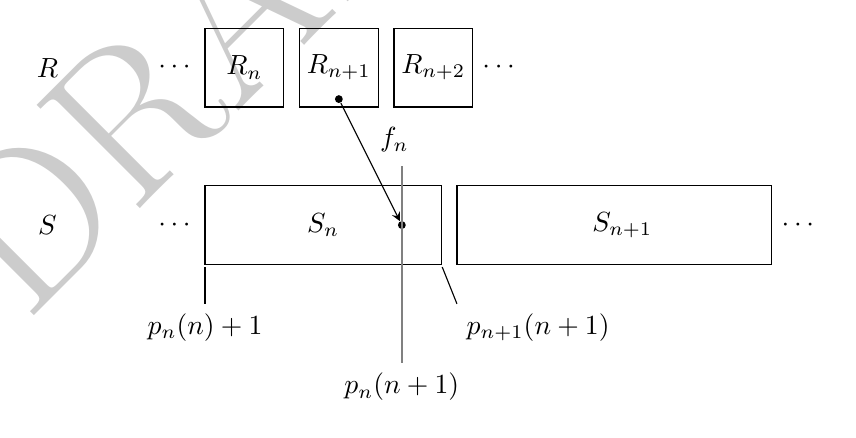
\begin{tikzpicture}[yscale=0.5]
        \begin{scope}[shift={(0, 5)}]
          \node at (0, 1) {$R$};

          %% Rectangles for equivalence classes of $R$.
          \draw (2, 0)
          %% TODO should be a way to use [current node is local] option here...
          ++(0, 1) node[anchor=east] {$\dotsb$} ++(0, -1)
          rectangle ++(1, 2)
          ++(0.2, -2)
          rectangle ++(1, 2)
          ++(0.2, -2)
          rectangle ++(1, 2)
          ++(0, -1)
          node[anchor=west] {$\dotsb$}
          ;

          %% Labels for each equivalence class of $R$.
          \path
          (2.5, 1) node {$R_n$}
          ++(1.2, 0) node {$R_{n + 1}$}
          ++(1.2, 0) node {$R_{n + 2}$}
          ;
        \end{scope}

        %% Arrow from top to bottom showing image under $f_n$.
        \begin{scope}[shift={(0, 1)}]
          \draw
          (4.5, 1) node[shape=circle, fill=black, inner sep=1pt] (source) {}
          ++(-0.8, 3.2) node[shape=circle, fill=black, inner sep=1pt] (target) {};
          \path[<-, >=stealth] (source) edge node[anchor=south west] {$f_n$} (target);
        \end{scope}

        \begin{scope}[shift={(0, 1)}]
          \node at (0, 1) {$S$};

          %% Rectangles for equivalence classes of $S$.
          \draw (2, 0)
          %% TODO should be a way to use [current node is local] option here...
          ++(0, 1) node[anchor=east] {$\dotsb$} ++(0, -1)
          rectangle ++(3, 2)
          ++(0.2, -2)
          rectangle ++(4, 2)
          ++(0, -1)
          node[anchor=west] {$\dotsb$}
          ;

          %% Labels for each equivalence class of $S$.
          \path
          (3.5, 1) node {$S_n$}
          ++(3.8, 0) node {$S_{n + 1}$}
          ;
        \end{scope}

        %% Labels underneath each $S_i$ showing length bounds.
        \begin{scope}
          \draw[shorten >=1pt]
          (2, 0) node[anchor=north] (pn) {$p_n(n) + 1$}
          -- ++(0, 1);
          \draw[thick, color=gray] (4.5, 3.5)
          -- ++(0, -5)
          node[anchor=north, color=black] (pnplus1) {$p_n(n + 1)$}
          ;
          \draw[shorten >=1pt]
          (5.2, 0) node[anchor=north west, color=black] (pnplus1nplus1) {$p_{n + 1}(n + 1)$}
          -- ++(-0.2, 1);
          ;
        \end{scope}
      \end{tikzpicture}
    \end{center}
  \end{figure}

  Finally, we show that $R$ and $S$ are in $\NC^1$.
  Deciding whether two strings have the same length is trivial, so $R$ is certainly in $\NC^1$.
  To decide $S$, we compute the index $i$ of the equivalence class $S_i$ containing the string $x$ and the index $j$ of the equivalence class $S_j$ containing the string $y$, then compare them for equality.
  Computing the index $i$ of the equivalence class of a string $x$ of length $n$ can be performed as follows.
  First, compute in parallel the values $p_1(1), \dotsc, p_{n + 1}(n + 1)$.
  Since each $p_i$ is increasing, $n$ is definitely smaller than $p_{n + 1}(n + 1)$.
  Computing the exponentiation of $O(n)$ pairs of strings of length $O(n)$ each can be performed by a $\TC^0$ circuit, and $\TC^0 \subseteq \NC^1$.
  Next, for each $i \in \{1, \dotsc, n\}$ in parallel, decide if $p_i(i) + 1 \leq n \leq p_{i + 1}(i + 1)$, thereby determining whether the input is in $S_i$.
  These comparisons can be performed by an $\NC^1$ circuit.
  Finally, use $O(\log n)$ single-bit multiplexers in parallel to output the index (in binary) of the sole equivalence class $S_i$ containing $x$.
  A single-bit multiplexer for $O(\log n)$ input bits can be implemented by a circuit of size $O(\log n)$ and depth $O(\log \log n)$ \autocite[Lemma~2.5.5]{savage98}, so this phase of the computation can be performed by an $\NC^1$ circuit.
  Computing the indices $i$ and $j$ for the two input strings can be performed in parallel, and the final comparison for equality of $i$ and $j$ adds only $O(\log n)$ depth to the circuit.
  Therefore $S \in \NC^1$.
\end{proof}

%%%%
%% generalcompleteness.tex
%%
%% Copyright 2011, 2012 Jeffrey Finkelstein
%%
%% Except where otherwise noted, this work is made available under the terms of
%% the Creative Commons Attribution-ShareAlike 3.0 license,
%% http://creativecommons.org/licenses/by-sa/3.0/.
%%
%% You are free:
%%    * to Share — to copy, distribute and transmit the work
%%    * to Remix — to adapt the work
%% Under the following conditions:
%%    * Attribution — You must attribute the work in the manner specified by
%%    the author or licensor (but not in any way that suggests that they
%%    endorse you or your use of the work).
%%    * Share Alike — If you alter, transform, or build upon this work, you may
%%    distribute the resulting work only under the same, similar or a 
%%    compatible license.
%%    * For any reuse or distribution, you must make clear to others the 
%%    license terms of this work. The best way to do this is with a link to the
%%    web page http://creativecommons.org/licenses/by-sa/3.0/.
%%    * Any of the above conditions can be waived if you get permission from
%%    the copyright holder.
%%    * Nothing in this license impairs or restricts the author's moral rights.
%%%%
\section{Conditions for complete problems under polynomial time kernel reductions}
\label{sec:generalcompleteness}

In this section we use the techniques of \cite[Theorem~8.7]{bcffm} to present a general theorem which provides equivalence relations which are hard for a number of interesting complexity classes under polynomial time kernel reductions.
We need one additional definition here.
If $\mathcal{C}$ is a complexity class then the class $\forall\mathcal{C}$ is the set of languages $A$ such that there exists a language $B\in\mathcal{C}$ and a polynomial $p$ satisfying $x\in A$ if and only if $\forall w\in\Sigma^{\leq p(|x|)} \pair{x}{w}\in B$.
$\forall\mathcal{C}$ is called the \defn{closure of $\mathcal{C}$ under polynomially bounded universal quantification}.

\begin{theorem}\label{thm:generalcompleteness}
  \printcompletenesstheorem
\end{theorem}

Before proving this theorem, we will provide some immediate corollaries of this general result.

\begin{corollary}
  If $\mathcal{C}$ is a subset of $\PSPACE$ and $\mathcal{C}=\CRAZY$, then $\CEq$ has a complete problem under $\kr$ reductions.
\end{corollary}

\begin{corollary}\label{cor:hardproblems}
  Under polynomial time kernel reductions,
  \begin{enumerate}
  %\item $\EXPEq$ has a complete problem
  \item $\PSPACEEq$ has a complete problem
  \item\label{itm:hardforsigma} $\PKPOPEq$ contains a problem which is hard for $\SKPEq$, for all $k\geq 0$
  \item $\PKPOPEq$ contains a problem which is hard for $\PKPEq$, for all $k\geq 0$
  %\item $\coNPEq$ contains a problem which is hard for $\PEq$
  \end{enumerate}
\end{corollary}
\begin{proof}\mbox{}
  \begin{enumerate}
  %\item $\EXP$ is closed under complement (because it is a deterministic complexity class) and polynomially bounded universal quantification (because we can simulate the universal guess deterministically in exponential time).
  \item $\PSPACE$ is closed under complement (because it is a deterministic complexity class) and polynomially bounded universal quantification (because we can simulate the universal guess deterministically in polynomial space).
  \item If $\mathcal{C}=\SKP$, then the $\kr$-hard problem is in $(\forall(\SKP\cup\mathsf{co}\SKP))\mathsf{Eq}=(\forall(\SKP\cup\PKP))\mathsf{Eq}=\PKPOPEq$.
  \item Same as the previous justification, but starting with $\mathcal{C}=\PKP$.\qedhere
%  \item Same as the previous justification, but starting with $\mathcal{C}=\P$.
  \end{enumerate}
\end{proof}

More specifically, this means that $\coNPEq$ has a problem which is $\kr$-hard for $\PEq$.
\autoref{cor:hardproblems} also implies part 1 of \cite[Theorem~8.7]{bcffm}, which is restated here.

\begin{corollary}[\cite{bcffm}, Theorem~8.7, part 1]
  If $\NP=\coNP$ then $\NPEq$ has a complete problem under polynomial time kernel reductions.
\end{corollary}
\begin{proof}
  If $\NP=\coNP$, then the polynomial hierarchy collapses, and specifically $\mathsf{\Pi_2P}=\mathsf{\Pi_1P}=\coNP=\NP$.
  From \autoref{itm:hardforsigma} in \autoref{cor:hardproblems} we conclude that $\NPEq$ has a $\kr$-hard problem for $\NPEq$.
  Such a problem is by definition $\NPEq$-complete.
\end{proof}

We now return to the proof of \autoref{thm:generalcompleteness} by first providing some motivating ideas.
Recall the canonical complete problem (sometimes called the ``universal'' problem) for $\NP$ (and indeed for various other complexity classes):
\begin{displaymath}
  K = \lb\triple{M}{x}{1^t} \st M\plain{accepts} x \plain{within} t \textnormal{ steps}\rb
\end{displaymath}
The idea of this proof is to adapt this into an equivalence relation $R_K$ consisting of pairs of triples of the form $\pair{\triple{M}{x}{1^{t_x}}}{\triple{M}{y}{1^{t_y}}}$, where $M$ accepts $\pair{x}{y}$, as in the reduction from an arbitrary $\NP$ language to $K$.
The problem we encounter here is that $R_K$ is not necessarily an equivalence relation.
Consider, for example, transitivity, which must be satisfied for all possible pairs of the form $\triple{M}{w}{1^{t_w}}$.
For \emph{arbitrary machines} $M$, just because $M$ accepts $\pair{x}{y}$ and $\pair{y}{z}$ does not necessarily mean that $M$ accepts $\pair{x}{z}$.
The solution is to encode into $R_K$ the requirement that the language which $M$ accepts, $L(M)$, is itself an equivalence relation.
The three properties required of $R_K$ then follow from the properties of $L(M)$.
%
%As a technical consideration for this proof, we point out languages in $\PSPACE$ may be decided by alternating Turing machines which run in polynomial time, so it is permissible to consider polynomially clocked Turing machines.
%
\begin{proof}[Proof of \autoref{thm:generalcompleteness}]
  First we will define a helper algorithm which decides whether a given machine accepts an equivalence relation on strings up to a given length.
  Define the algorithm $A$ as follows on input $\pair{M}{n}$, where $M$ is a polynomially clocked Turing machine of type $\mathcal{C}$ and $n\in\mathbb{N}$:
  \begin{enumerate}
  \item universally guess $a,b,$ and $c\in\Sigma^{\leq n}$
  \item simulate $M$ on $\pair{a}{a}$; if it rejects, reject
  \item simulate $M$ on $\pair{a}{b}$, then on $\pair{b}{a}$; if the former accepts and the latter rejects, reject
  \item simulate $M$ on $\pair{a}{b}$, then on $\pair{b}{c}$, then on $\pair{a}{c}$; if the first two accept and the last one rejects, reject
  \item if execution reaches this point, accept
  \end{enumerate}
  These simulations check that $L(M)$ satisfies reflexivity, symmetry, and transitivity on strings of length at most $n$.
  If $A$ accepts, then the three properties are satisfied, and if it rejects then one of the three properties is violated.
  Since $M$ is a machine of type $\mathcal{C}$, checking if $M$ accepts on some input and if $M$ rejects on some input is in $\mathcal{C}\cup\mathsf{co}\mathcal{C}$.
  The universal guesses of $a,b,$ and $c$ (of length at most $n$) followed by checks of whether the six simulations of $M$ accept or reject place $L(A)$ in the class $\CRAZY$.
  If $p$ is the polynomial which bounds the running time of $M$, then the running time of this algorithm is $6p(|\pair{1^n}{1^n}|)+c$, where $c$ is a constant which represents the time needed to account for the implementation of $A$ (the control of the simulations of $M$, performing logical conjunctions, etc.).
  Hence the running time of $A$ is polynomial in $n$.

  Now we can define the set $R_K$ by
  \begin{align*}
    R_K = {} & \lb\pair{u}{v} \st u=v\rb \\
    & \cup \lb\pair{\triple{M}{x}{1^{t_x}}}{\triple{M}{y}{1^{t_y}}} \st \textnormal{1 through 4 below are satisfied}\rb
  \end{align*}
  where the conditions are
  \begin{enumerate}
  \item\label{itm:machine} $M$ is a polynomially clocked Turing machine of type $\mathcal{C}$
  \item\label{itm:emx} $A$ accepts $\pair{M}{|x|}$ within $t_x$ steps
  \item\label{itm:emy} $A$ accepts $\pair{M}{|y|}$ within $t_y$ steps
  \item\label{itm:accepts} $M$ accepts $\pair{x}{y}$
  \end{enumerate}
  We claim that $R_K$ is in $\CRAZYEq$ and $\CEq$-hard.

  First we show that $R_K\in\CRAZY$.
  By the argument above, $A$ is a $\CRAZY$ algorithm.
  %Since $M$ is a polynomially clocked $\mathcal{C}$ machine by \autoref{itm:machine}, then the simulation of $M$ on $\pair{x}{y}$ in \autoref{itm:accepts} can be performed by a $\mathcal{C}$ algorithm.
  Assuming without loss of generality that $|x|\geq |y|$, if $A$ accepts $\pair{M}{|x|}$ within $t_x$ steps then we know that there is a polynomial time bound on the running time of $M$ on input $\pair{x}{y}$, so simulating it is certainly in $\CRAZY$.
  Finally, testing for equality is in $\mathcal{C}$ by hypothesis so deciding $R_K$ overall can be performed by a $\CRAZY$ algorithm.

  Next we show that $R_K$ is an equivalence relation.
  Reflexivity follows from the reflexivity of the equality relation.
  For symmetry, suppose $\pair{\triple{M}{x}{1^{t_x}}}{\triple{M}{y}{1^{t_y}}}\in R_K$.
  Since \autoref{itm:emx} and \autoref{itm:emy} are true by hypothesis, we know that symmetry on strings of length at most $\max(|x|, |y|)$ in $L(M)$ is satisfied, and that includes the strings $x$ and $y$.
  So since $M$ accepts $\pair{x}{y}$ it must follow that $M$ accepts $\pair{y}{x}$.
  Furthermore, \autoref{itm:machine}, \autoref{itm:emx}, and \autoref{itm:emy} are the same up to symmetry of $x$ and $y$, so we have $\pair{\triple{M}{y}{1^{t_y}}}{\triple{M}{x}{1^{t_x}}}\in R_K$.
  For transitivity, suppose that both $\pair{\triple{M}{x}{1^{t_x}}}{\triple{M}{y}{1^{t_y}}}\in R_K$ and $\pair{\triple{M}{y}{1^{t_y}}}{\triple{M}{z}{1^{t_z}}}\in R_K$.
  Since transitivity is true on strings of length at most $\max(|x|, |y|, |z|)$ by the transitivity propositions checked by \autoref{itm:emx} and \autoref{itm:emy}, and since $M$ accepts both $\pair{x}{y}$ and $\pair{y}{z}$ by hypothesis, it must follow that $M$ accepts $\pair{x}{z}$.
  Again the conditions in \autoref{itm:machine}, \autoref{itm:emx}, and \autoref{itm:emy} are the same.
  We have shown that $R_K$ is reflexive, symmetric, and transitive, so it is an equivalence relation.
  At this point, we have proven that $R_K\in\CRAZYEq$.

  Now we need to show that $R_K$ is $\CEq$-hard.
  Let $S\in\CEq$.
  Suppose $M$ is the polynomially clocked $\mathcal{C}$ machine which decides $S$, and $p$ is the polynomial which bounds the running time of $M$.
  Then the kernel reduction from $S$ to $R_K$ is $w\mapsto\triple{M}{w}{1^{6p(|\pair{w}{w}|)+c}}$, where $p$ and $c$ are the polynomial and constant described in the first paragraph of this proof.
  Call this reduction $f$.
  The reduction is obviously computable in time polynomial in $|w|$.
  It remains to show that this reduction is correct.

  Suppose $\pair{x}{y}\in S$.
  Now $f(x)=\triple{M}{x}{1^{6p(|\pair{x}{x}|)+c}}$ and $f(y)=\triple{M}{y}{1^{6p(|\pair{y}{y}|)+c}}$.
  \autoref{itm:machine} is true by construction, and \autoref{itm:accepts} is true since $M$ is the machine which decides $S$.
  Assume \autoref{itm:emx} is false.
  Then $M$ does not accept an equivalence relation on strings of length at most $|x|$.
  This is a contradiction, since $M$ decides $S$, an equivalence relation, by hypothesis.
  Therefore \autoref{itm:emx} must be satisfied.
  The same argument applies to \autoref{itm:emy}.
  Hence $\pair{f(x)}{f(y)}\in R_K$.

  If $\pair{x}{y}\notin S$ then $M$ does not accept $\pair{x}{y}$, since otherwise $\pair{x}{y}$ would be a member of $S$.
  Hence $\pair{x}{y}\notin R_K$.
  Therefore we have shown that $R_K$ is $\CEq$-hard.
\end{proof}

\begin{openproblem}
  Is there a more general characterization of complexity classes which have a $\kr$-hard problem?
\end{openproblem}

\begin{openproblem}
  Under what conditions does a complexity class have a complete problem?
  Can we adapt this idea to create a complete problem for $\PEq$ or $\NPEq$?
\end{openproblem}

\begin{openproblem}
  Can this theorem be used to construct $\krnt$-hard problems for smaller complexity classes like $\NLEq$ under the appropriate time-bounded reduction?
  Larger classes such as $\EXPEq$?
\end{openproblem}

\begin{openproblem}
  To what other equivalence relations does our $\kr$-hard problem reduce?
  Are there ``natural'' $\kr$-hard problems in complexity classes which satisfy the conditions in \autoref{thm:generalcompleteness}?
\end{openproblem}

As an additional corollary, we show that the equivalence relation $R_K$ is necessarily hard given a known hard equivalence relation under $\kr$ reductions.

\begin{corollary}
  Let $\mathcal{C}_1$ be a complexity class and $\mathcal{C}_2$ be a subset of $\PSPACE$ which contains the problem of deciding whether two strings are equal.
  If there exists an equivalence relation $S$ in $\CTEq$ which is hard for $\COEq$ under $\kr$ reductions, then there is an equivalence relation in $\CRAZIEREq$ which is hard for $\COEq$ under $\kr$ reductions.
\end{corollary}
\begin{proof}
  $S\kr R_K$ by the reduction described in the proof of \autoref{thm:generalcompleteness}.
  A similar analysis shows that $R_K\in\CRAZIEREq$.
  Since $S$ is hard for $\COEq$ and polynomial time kernel reductions compose by \autoref{prop:compose}, $R_K$ is also hard for $\COEq$.
\end{proof}

Finally, the following theorem is inspired by Mahaney's theorem, which states that there are no sparse \NP-complete languages unless $\P=\NP$.
Our result concerns not the sparseness of strings in a language, but the sparseness of equivalence classes in an equivalence relation.
This complements the work on ``potential reducibility'', defined in section 5 of \cite{bcffm}.

\begin{definition}[\cite{bcffm}, Definition~7.2]
  \mbox{}
  \begin{enumerate}
  \item If $R$ is an equivalence relation on $\Sigma^*$, then define $\#R(n)$ to be $\left|\{[x]_R | x \in \Sigma^{\leq n}\}\right|$, or in other words, $\#R(n)$ is the number of equivalence classes in $R$ for strings of length at most $n$.
  \item
    Let $R$ and $S$ be equivalence relations on $\Sigma^*$.
    $R$ is \defn{potentially reducible} to $S$, denoted $R\pot S$, if there exists a polynomial $p$ such that for all $n\in\mathbb{N}$, $\#R(n)\leq \#S(p(n))$.
  \end{enumerate}
\end{definition}

It follows from the definitions that for any equivalence relations $R$ and $S$, $R\kr S\implies R\pot S$, and hence $R\npot S \implies R\nkr S$ (this is stated and proven explicitly in \cite[Lemma~5.5]{bcffm}).
As an analog to traditional sparse languages, we provide a definition of ``kernel sparsity'', and show its application to determining potential reducibility and hence kernel reducibility.

\begin{definition}
  An equivalence relation $R$ on $\Sigma^*$ is \defn{kernel sparse} if there exists a polynomial $p$ such that for all $n\in\mathbb{N}$, $\#R(n)\leq p(n)$.
  In other words, the number of equivalence classes in $R$ for strings of length at most $n$ is bounded above by a polynomial in $n$.

  An equivalence relation is \defn{kernel dense} if it is not kernel sparse.
  Formally, if for all polynomials $p$ there exists an $n\in\mathbb{N}$ such that $\#R(n)>p(n)$.
  In other words, the number of equivalence classes in $R$ for strings of length at most $n$ is greater than any polynomial in $n$.
\end{definition}

These definitions allow us to provide the following very natural proposition.
Intuitively, it states that an equivalence relation with many closely packed equivalence classes cannot reduce (under polynomially bounded notions of reduction) to an equivalence relation with few but widely spaced equivalence classes.

\begin{theorem}\label{prop:density}
  Let $R$ and $S$ be equivalence relations on $\Sigma^*$.
  If $R$ is kernel dense and $S$ is kernel sparse, then $R\npot S$ and in particular $R\nkr S$.
\end{theorem}
\begin{proof}
  That $R\npot S$ implies $R\nkr S$ was already stated in the text following the definition of potential reducibility, so it suffices to show that $R\npot S$.

  Assume that $R\pot S$ with the intention of producing a contradiction.
  Let $p$ be the polynomial such that $\#R(n)\leq \#S(p(n))$ (this is the definition of potential reducibility).
  Let $q$ be the polynomial such that for all $n$, $\#S(n)< q(n)$ (this is the definition of kernel sparse).
  %% TODO is this true?
  Assume without loss of generality that $q$ is non-decreasing (we can do this because for each polynomial $a$ there exists a non-decreasing polynomial $b$ such that $a(n)\leq b(n)$ for all $n$).
  For each natural number $n$, we have $\#S(n) \leq q(0) + q(1) + \cdots + q(n) \leq n \cdot q(n)$ (since $q$ is non-decreasing).
  Replacing $n$ with $p(n)$ in the above inequality, it follows that $\#S(p(n)) \leq p(n) \cdot q(p(n))$, which is a polynomial in $n$.
  (This is an overestimate, but we can be generous here and still produce a contradiction.)
  Let $r(n)=p(n)\cdot q(p(n))$.

  Let $n_0$ be the natural number such that $\#R(n_0) > r(n_0)$, by the definition of kernel sparse.
  Since $\#S(p(n_0)) \leq r(n_0)$, we have $\#R(n_0) > \#S(p(n_0))$.
  In other words, there are more equivalence classes in $R$ for strings up to length $n_0$ than there are in $S$ for strings up to length $p(n_0)$.
  By the pigeonhole principle, we conclude that $R$ cannot potentially reduce to $S$, because the number of equivalence classes in $R$ for strings up to length $n_0$ is too great compared to the number of equivalence classes in $S$ for strings up to length $p(n_0)$.
  This is a contradiction with the assumption that $R\pot S$.
  We have shown this for arbitrary polynomials (which came from the definitions of potential reducibility and kernel sparsity), so we can conclude that the result holds for all equivalence relations $R$ and $S$ which are kernel dense and kernel sparse, respectively.
\end{proof}

This places a strong restriction on equivalence relations which are hard (or complete) under polynomial time kernel reductions: they cannot be kernel sparse.

\begin{corollary}
  Let $\CEq$ be a complexity class of equivalence relations containing the equality relation, $R_{eq}=\lb\pair{x}{y} \st x=y\rb$.
  If an equivalence relation $R$ is $\CEq$-hard then it is not kernel sparse (that is, it is kernel dense).
\end{corollary}
\begin{proof}
  $R_{eq}$ is kernel dense since it contains $2^n$ equivalence classes at each length $n$---one for each distinct string.
  If $R$ were kernel sparse then $R_{eq}\npot R$ by \autoref{prop:density}.
  This would imply $R_{eq}\nkr R$, which is a contradiction with the hypothesis that all equivalence relations in $\CEq$ (including $R_{eq}$) polynomial time kernel reduce to $R$.
  Therefore $R$ is not kernel sparse.
\end{proof}

%% This last question leads us to briefly note that equivalence of true quantified boolean formulas is a \PSPACE-complete problem; perhaps it is also a \PSPACEEq-complete problem.
%% \begin{proposition}
%%   Define $\QBFEq$ by
%%   \begin{displaymath}
%%     \QBFEq = \{\pair{\phi}{\psi} | \phi \iff \psi\},
%%   \end{displaymath}
%%   where $\phi$ and $\psi$ are fully quantified boolean formulae.
%%   Then $\QBFEq$ is \PSPACE-complete.
%% \end{proposition}
%% \begin{proof}
%%   Suppose $\phi$ denotes $\overline{Q}\tau$, where $\overline{Q}$ represents the sequence of quantified variables and $\tau$ is the boolean formula over those variables.
%%   Then the many-one reduction from $\QBF$ is $\phi\mapsto\pair{\phi}{\exists z\colon\overline{Q}(\tau\land z)}$, where $z$ is a variable not already in $\phi$.
%%   This reduction can obviously be computed in time polynomial in the length of the input, $\phi$.
%%   If $\phi$ is not satisfiable, then no assignment of $z$ makes $\overline{Q}(\tau\land z)$ satisfiable, because $\tau$ will always be false.
%%   Hence $\exists z\colon\overline{Q}(\tau\land z)$ must be false.
%%   If $\phi$ is satisfiable, then choosing $z$ to be true makes $\overline{Q}(\tau\land z)$ true.
%%   Thus $\phi$ is satisfiable if and only if $\exists z\colon\overline{Q}(\tau\land z)$ is satisfiable, so $\QBF\mor\QBFEq$.
%%   Since $\QBFEq$ is clearly decidable in $\PSPACE$, we conclude that $\QBFEq$ is \PSPACE-complete.
%% \end{proof}

%% npeqcompleteness.tex - completeness in NP equivalence classes
%%
%% Copyright 2010, 2011, 2012, 2014, 2015 Jeffrey Finkelstein.
%%
%% This LaTeX markup document is made available under the terms of the Creative
%% Commons Attribution-ShareAlike 4.0 International License,
%% https://creativecommons.org/licenses/by-sa/4.0/.
\section
    [Relationship between completeness under kernel and many-one reductions]
    {Relationship between completeness \\ under kernel and many-one reductions}
\label{sec:npeqcompleteness}
% Foreword
%
% context (focus on anyone) why now? - current situation, and why the need is so important
A kernel reduction implies a many-one reduction, but does completeness under kernel reductions imply completeness under many-one reductions?
% need (focus on readers) why you? - why this is relevant to the reader, and why something needed to be done
Since polynomial time kernel reductions are different from polynomial time many-one reductions (\autoref{thm:different}), completeness in classes of equivalence problems may differ under these reductions as well.
% task (focus on author) why me? - what was undertaken to address the need
We determine the conditions under which completeness under kernel reductions implies completeness under many-one reductions.
% object (focus on document) why this document - what the document covers
%This section presents some information about the relationship between these two types of reductions.

% Summary
%
% findings (focus on author) what? - what the work revealed when performing the task
We find that completeness under many-one reductions follows as a straightforward consequence of completeness under kernel reductions as long as the relevant complexity class admits a complete problem under many-one reductions.
We also show that the kernel reduction is essentially too weak to allow for completeness under injective (that is, ``one-to-one'') reductions, for combinatorial reasons similar to those in \autoref{sec:limitations}.
Though we prove these results for $\NPEq$, they generalize in a natural way to any ``well-behaved'' complexity class (basically, any class containing a complete problem under many-one reductions).
% conclusion (focus on readers) so what? - what the findings mean for the audience
These results are more indication that when comparing the relative difficulty of equivalence problems, one should attempt to construct a kernel reduction instead of a many-one reduction.
% perspective (focus on anyone) what now? - what should be done next
The potential lack of a complete problem under injective kernel reductions suggests that a conjecture analagous to the Berman--Hartmanis conjecture, which states that all $\NP$-complete problems are isomorphic with respect to many-one reductions, may be false in $\NPEq$.

Let \textsc{GI} denote the equivalence relation consisting of all pairs of isomorphic graphs.
A property, that is, a Boolean function, $\Pi$ is an \defn{$\NP$-complete property} if $L_\Pi$, the set of all strings for which $\Pi$ is true, is $\NP$-complete.
If, furthermore, the property satisfies $\pair{x}{y} \in R$ implies $\Pi(x) = \Pi(y)$ where $R$ is an equivalence relation, $\Pi$ is called a \emph{property on $R$}.
For example, Hamiltonicity, the property of having a cycle that includes each vertex, is an $\NP$-complete property on \textsc{GI}.

\begin{theorem}\label{thm:npceqrel}
  If $\Pi$ is an \NP-complete property on \textsc{GI}, then the equivalence relation $A$ defined by
  \begin{equation*}
    A = \left\{ \pair{G}{H} \, \middle| \, \pair{G}{H} \in \textsc{GI} \text{ or } (G \in L_\Pi \text{ and } H \in L_\Pi) \right\}
  \end{equation*}
  is an \NP-complete equivalence relation.
\end{theorem}
\begin{proof}
  It is straightforward to prove that $A$ is an equivalence relation, so it remains to show that it is $\NP$-complete.
  The language $A$ is in $\NP$ because both $R$ and $L_\Pi$ are in $\NP$ by hypothesis.
  Thus we need only show that $A$ is $\NP$-hard.

  Let $H$ be a graph satisfying $\Pi$; such a graph must exist because $\Pi$ is $\NP$-complete and therefore there must be at least one graph that satisfies $\Pi$ and at least one that does not (otherwise no many-one reduction to $L_\Pi$ could exist).
  The reduction proving that $A$ is $\NP$-complete is from $L_\Pi$, and the mapping is given by $G \mapsto \pair{G}{H}$.
  This function is computable in linear time; the size of $H$ is constant with respect to the size of $G$.

  Now we show that $G \in L_\Pi$ if and only if $\pair{G}{H} \in A$, for any graph $G$.
  If $G \in L_\Pi$, then $G \in L_\Pi$ and $H \in L_\Pi$, so $\pair{G}{H} \in A$.
  If $\pair{G}{H} \in A$, then either $G \in L_\Pi$ and $H \in L_\Pi$, in which case $G \in L_\Pi$, or $G$ is isomorphic to $H$, in which case $G$ is in $L_\Pi$ because $H$ is.
  In either case $G \in L_\Pi$.
  We conclude that $L_\Pi \mor A$, and so $A$ is an $\NP$-complete equivalence relation.
\end{proof}

\begin{example}\label{ex:npceqrel}
  The language
  \begin{equation*}
    \left\{ \pair{G}{H} \, \middle| \, \pair{G}{H} \in \textsc{GI} \text{ or } G \text{ and } H \text{ have a Hamiltonian cycle}  \right\}
  \end{equation*}
  is an \NP-complete equivalence relation.
\end{example}

\begin{corollary}
  If $R$ is $\NPEq$-complete, then $R$ is $\NP$-complete.
\end{corollary}
\begin{proof}
  Let $A$ denote the $\NP$-complete equivalence relation defined in \autoref{ex:npceqrel}.
  Since $R$ is $\NPEq$-complete by hypothesis, $A \kr R$.
  Since a kernel reduction implies a many-one reduction, $R$ is also $\NP$-complete.
\end{proof}

This corollary provides a clearer proof of \autocite[Proposition~8.1]{bcffm}.

\begin{corollary}[{\autocite[Proposition~8.1]{bcffm}}]
  If \textsc{GI} is \NPEq-complete then the polynomial hierarchy collapses to the second level ($\PH = \STP$).
\end{corollary}
\begin{proof}
  By the previous corollary, if \textsc{GI} is $\NPEq$-complete, then it is $\NP$-complete, which implies the stated collapse (see \autocite{schoning87}).
\end{proof}

\autoref{thm:npceqrel} also provides a simple method for proving the equivalence of $\P = \NP$ and $\PEq = \NPEq$.

\begin{theorem}\label{thm:pnppeqnpeq}
  $\P = \NP$ if and only if $\PEq = \NPEq$.
\end{theorem}
\begin{proof}
  If $\P = \NP$, then $\PEq = \NPEq$ by their definitions.
  Suppose now that $\PEq = \NPEq$.
  Let $A$ denote the $\NP$-complete equivalence relation defined in \autoref{ex:npceqrel}.
  Since $A \in \NPEq$ and $\PEq = \NPEq$ by hypothesis, $A \in \PEq$, and hence $A \in \P$.
  Since $\P$ is closed under $\mor$ reductions, any $\NP$-complete problem in $\P$ implies $\P = \NP$.
\end{proof}

As stated in \autoref{open:npeqc}, we do not know whether an $\NPEq$-complete problem exists.
In the following theorem we describe an equivalence relation that, if it were $\NPEq$-complete, would prove that injective kernel reductions are strictly weaker than general kernel reductions.
This is interesting because it again demonstrates that the number and size of equivalence classes is important when considering the (im)possibility of polynomial time kernel reductions between equivalence relations.
In the following theorem, if an equivalence relation is ``complete under $\kri$ reductions in $\NPEq$'' we mean that every equivalence relation in $\NPEq$ reduces to it by a polynomial time computable kernel reduction which is also injective (that is, ``one-to-one'').

\begin{theorem}\label{thm:inj}
  Let $\Pi$ be a property on \textsc{GI}.
  %% If for each natural number $n$ there is a graph $G$ of size $n$ such that $\Pi(G) = 1$, and 
  If the equivalence relation $A$ defined by
  \begin{equation*}
    A = \left\{ \pair{G}{H} \, \middle| \, \pair{G}{H} \in \textsc{GI} \text{ or } (G \in L_\Pi \text{ and } H \in L_\Pi \text{ and } |G| = |H|) \right\}
  \end{equation*}
  is complete for $\NPEq$ under $\kr$ reductions, then $A$ is not complete under $\kri$ reductions.
\end{theorem}

The only difference between the equivalence relation $A$ defined here and the one defined in \autoref{thm:npceqrel} is the requirement that $|G| = |H|$.
This means that although the number of equivalence classes in $A$ is infinite (at least one for each size), each of those equivalence classes is itself finite.
In contrast, consider the equivalence relation $S$ defined by
\begin{equation*}\label{eq:ones}
  S = \left\{ \pair{x}{y} \, \middle| \, x \text{ and } y \text{ have the same number of } 1 \text{s} \right\}.
\end{equation*}
The equivalence relation $S$ has an infinite number of equivalence classes: $[1]$, $[11]$, $[111]$, etc.
Each equivalence class is itself infinite as well: for each $w \in \Sigma^*$, the equivalence class $[w]$ contains $w$, $0w$, $00w$, etc.

\begin{proof}[Proof of \autoref{thm:inj}]
  Let $S$ be the equivalence relation defined in the preceding paragraph.
  The language $S$ is decidable in linear time by a deterministic Turing machine, hence it is in $\NP$.
  Since $A$ is $\NPEq$-complete by hypothesis, $S \kr A$.
  Thus there is a polynomial time computable function $f$ such that $\pair{x}{y} \in S$ if and only if $\pair{f(x)}{f(y)} \in A$.

  By the discussion preceding this theorem, $[w]_S$ is infinite and $[f(w)]_A$ is finite.
  By \autoref{lem:image}, $f([w]_S) \subseteq [f(w)]_A$.
  Consider $f|_{[w]_S}$, that is, $f$ restricted to the domain $[w]_S$.
  Then $f|_{[w]_S}$ is a mapping from the infinite set $[w]_S$ to the finite set $[f(w)]_A$.
  By the pigeonhole principle, $f|_{[w]_S}$ is not injective.
  Hence the unrestricted reduction $f$ is not injective, and therefore $A$ is not $\kri$-complete in $\NPEq$.
\end{proof}

%% intermediary.tex - NP-intermediary equivalence relations
%%
%% Copyright 2010, 2011, 2012, 2014, 2015 Jeffrey Finkelstein.
%%
%% This LaTeX markup document is made available under the terms of the Creative
%% Commons Attribution-ShareAlike 4.0 International License,
%% https://creativecommons.org/licenses/by-sa/4.0/.
\section{Existence of intermediary problems}
\label{sec:intermediary}
% Foreword
%
% context (focus on anyone) why now? - current situation, and why the need is so important
According to the seminal theorem by Ladner \autocite{ladner}, if $\P \neq \NP$, then there are problems of intermediate complexity, in the sense that these problems are neither in $\P$ nor $\NP$-complete.
The theorem does not immediately imply a similar result for equivalence problems, since $\PEq$ is different from $\P$ and $\NPEq$ is different from $\NP$ (specifically, in each case, the latter contains problems that are not equivalence problems).
% need (focus on readers) why you? - why this is relevant to the reader, and why something needed to be done
Do kernel reductions induce the same rich structure between $\PEq$ and $\NPEq$ as do many-one reductions between $\P$ and $\NP$?
% task (focus on author) why me? - what was undertaken to address the need
We adapt Schöning's Uniform Diagonalization Theorem \autocite{schoning}, a generalized version of Ladner's Theorem, to classes of equivalence problems.
The specific presentation we follow is from \autocite{bdg95}.
% object (focus on document) why this document - what the document covers
This section details the proof of that adaptation.

% Summary
%
% findings (focus on author) what? - what the work revealed when performing the task
The main theorem of this section, following as a corollary from the Uniform Diagonalization Theorem for equivalence problems, is as follows.
\begin{restatable*}{theorem}{intermediary}\label{thm:intermediary}
  If $\PEq \neq \NPEq$ and there is an $\NPEq$-complete problem, then there is an equivalence relation in $\NPEq$ that is neither in $\PEq$ nor $\NPEq$-complete.
\end{restatable*}
Although this theorem relies on the assumption that there is an $\NPEq$-complete problems, no such assumption is required to show the existence of intermediary problems between, say, $\PHEq$ and $\PSPACEEq$ (\autoref{cor:pspace}).
% conclusion (focus on readers) so what? - what the findings mean for the audience
We conclude that even though kernel reductions are strictly weaker than many-one reductions, they still preserve the hierarchies of problems of various computational complexities we expect from our understanding of traditional complexity classes.
% perspective (focus on anyone) what now? - what should be done next
The graph isomorphism problem, as one of the few candidates for an $\NP$-intermediary problem, may be the best candidate for an $\NPEq$-intermediary problem as well.

First we need to provide some technical definitions.

\begin{definition}
  A class of languages $\mathcal{C}$ is \defn{closed under finite variations} if and only if $A\in \mathcal{C}$ and $A\symdiff B$ (the symmetric difference of $A$ and $B$) is finite implies $B\in \mathcal{C}$ for all $B$.
\end{definition}

\begin{definition}
  The \defn{kernel join} of two equivalence relations $R$ and $S$, denoted $R \kj S$, is defined by
  \begin{equation*}
    R \kj S = \lb \pair{x0}{y0} \st \pair{x}{y} \in R \rb \cup \lb \pair{x1}{y1} \st \pair{x}{y} \in S \rb \cup \{(\lambda, \lambda)\}.
  \end{equation*}
\end{definition}

The pair of empty strings $(\lambda, \lambda)$ is required in the above definition so that the equivalence classes of $R \kj S$ partition the set of all finite strings $\Sigma^*$.

\begin{lemma}\label{lem:join}
  If $R$ and $S$ are equivalence relations, then $R \kj S$ is an equivalence relation.
\end{lemma}
\begin{proof}
  The proof follows immediately from the definitions.
  %% Since the equivalence class of the empty string, $[\lambda]$, is a singleton set, each of the three properties required of an equivalence relation hold for that set.
  %% Thus we need only consider nonempty strings.
  %% Let $x$, $y$ and $z$ be nonempty strings in $\Sigma^*$.
  %%
  %% Since $x$ is non-empty, $x = x'0$ or $x = x'1$.
  %% If $x = x'0$, then $\pair{x'}{x'} \in R$ since $R$ is reflexive.
  %% If $x = x'1$, then $\pair{x'}{x'} \in S$ since $R$ is reflexive.
  %% Hence $\pair{x}{x}\in R\kj S$ regardless of the last bit of $x$.
  %% Therefore $R \kj S$ is reflexive.
  %%
  %% Suppose $\pair{x}{y}\in R\kj S$.
  %% Then either $x=x'0$, $y=y'0$ and $\pair{x'}{y'}\in R$ or $x=x'1$, $y=y'1$ and $\pair{x'}{y'}\in S$.
  %% In either case, symmetry follows from the symmetry of $R$ or $S$.
  %%
  %% Suppose $\pair{x}{y}$ and $\pair{y}{z}$ are both in $R\kj S$.
  %% In the case that $x=x'0$, $y=y'0$ and $\pair{x'}{y'}\in R$, and that $z=z'0$ and $\pair{y'}{z'}\in R$, then by the transitivity of $R$, $\pair{x'}{z'}\in R$, so $\pair{x}{z}\in R\kj S$.
  %% The argument is similar in the case that $x=x'1$, $y=y'1$ and $z=z'1$.
  %% It is a contradiction for the other two cases to exist, since $y$ cannot be equal to both $y'0$ and $y'1$.
  %%
  %% Since $R\kj S$ is reflexive, symmetric and transitive, $R\kj S$ is an equivalence relation.
\end{proof}

\begin{proposition}\label{prop:symdiff}
  Symmetric difference of equivalence relations preserves symmetry.
\end{proposition}
\begin{proof}
  Let $R$ and $S$ be equivalence relations.
  Let $(x,y)\in(R\symdiff S)$.
  In the case that $(x,y)\in R$ and $(x,y)\notin S$, then $(y,x)\in R$.
  If $(y,x)$ were in $S$, then $(x,y)$ would also be in $S$, by symmetry, but this is a contradiction.
  Hence $(y,x)\in R$ and $(y,x)\notin S$.
  The argument for the other case is symmetric.
  Therefore $(x,y)\in(R\symdiff S)\implies (y,x)\in(R\symdiff S)$.
\end{proof}

\begin{definition}
  Let $r\colon\mathbb{N}\to\mathbb{N}$ be a computable function such that $r(m)>m$ for all $m$.
  Define the set $G[r]$ as
  \begin{displaymath}
    G[r]=\lb x\in\Sigma^* \st r^n(0)\leq|x|<r^{n+1}(0) \plain{for some even} n\rb
  \end{displaymath}
  where $r^n(m)$ denotes the $n$-fold application of $r$ to $m$:
  \begin{displaymath}
    \overbrace{r\circ r\circ r\circ\cdots\circ r}^{n \plain{times}}(m)
  \end{displaymath}
  $G[r]$ is called the \defn{gap language} generated by $r$.
\end{definition}

\begin{lemma}\label{lem:gap_p}
  If $r$ is time constructible, then $G[r]\in\P$.
\end{lemma}
\begin{proof}
  %% TODO add theorem number in this citation
  The proof can be found in \autocite{bdg95}.
\end{proof}

We will denote the Cartesian product $G[r]\times G[r]$ by the slightly more succinct ${G[r]}^2$, and $\overline{G[r]}\times\overline{G[r]}$ by $\overline{G[r]}^2$.
Elements of ${G[r]}^2$ are pairs of strings whose lengths are in the ``even gaps'' of $r$, while elements of $\overline{G[r]}^2$ are pairs of strings whose lengths are in the ``odd gaps'' of $r$.

\begin{lemma}
  ${G[r]}^2$ and $\overline{G[r]}^2$ are \defn{partial equivalence relations} (that is, they are symmetric and transitive).
\end{lemma}
\begin{proof}
  The proof follows immediately from the definitions.
  %% We will prove the theorem for ${G[r]}^2$; a symmetric argument proves the theorem for $\overline{G[r]}^2$.
  %%
  %% Let $x,y\in\Sigma^*$.
  %% Suppose $\pair{x}{y}\in {G[r]}^2$, so the lengths of $x$ and $y$ are both in an even gap of $r$.
  %% Then $\pair{y}{x}\in{G[r]}^2$, so ${G[r]}^2$ is symmetric.
  %% Now let $z\in\Sigma^*$ and suppose also that $\pair{y}{z}\in {G[r]}^2$.
  %% Then $y$ and $z$ are both in an even gap of $r$, so $x$, $y$ and $z$ are all in some even gap of $r$, and hence $\pair{x}{z}\in {G[r]}^2$.
  %% Therefore ${G[r]}^2$ is transitive.
\end{proof}

We are now prepared to prove the main technical theorem which will allow us to construct an equivalence relation which is ``between'' two complexity classes.

\begin{theorem}\label{thm:diag}
  Let $R_1$ and $R_2$ be decidable equivalence relations, and let $\mathcal{C}_1$ and $\mathcal{C}_2$ be classes of decidable equivalence relations such that
  \begin{enumerate}
  \item $R_1\notin\mathcal{C}_1$,
  \item $R_2\notin\mathcal{C}_2$,
  \item $\mathcal{C}_1$ and $\mathcal{C}_2$ are computably enumerable,
  \item $\mathcal{C}_1$ and $\mathcal{C}_2$ are closed under finite variations.
  \end{enumerate}
  Then there exists a decidable equivalence relation $R$ such that
  \begin{enumerate}
  \item $R\notin \mathcal{C}_1$,
  \item $R\notin \mathcal{C}_2$,
  \item $R\kr R_1\kj R_2$.
  \end{enumerate}
\end{theorem}
\begin{proof}
  Let $P_1, P_2, \ldots$ and $Q_1, Q_2, \ldots$ be enumerations of Turing machines deciding the languages in $\mathcal{C}_1$ and $\mathcal{C}_2$ respectively.
  Define the functions
  \begin{eqnarray*}
    r_1(n)=\underset{i\leq n}{max}\{|z_{i,n}|\}+1 & \text{and} &
    r_2(n)=\underset{i\leq n}{max}\{|z'_{i,n}|\}+1
  \end{eqnarray*}
  where $z_{i,n}$ is the smallest word in $\Sigma^*$ such that there exists an $x\in\Sigma^*$, with $n<|x|\leq|z_{i,n}|$, such that $\pair{z_{i,n}}{x}\in(L(P_i)\symdiff R_1)$, and $z'_{i,n}$ is the smallest word in $\Sigma^*$ such that there exists an $x'\in\Sigma^*$, with $n<|x'|\leq|z'_{i,n}|$, such that $\pair{z'_{i,n}}{x'}\in(L(Q_i)\symdiff R_2)$.
  Note that it also suffices to find an $x$ and $x'$ such that $\pair{x}{z_{i,n}}\in(L(P_i)\symdiff R_1)$ and $\pair{x'}{z'_{i,n}}\in(L(Q_i)\symdiff R_2)$, since symmetric difference on equivalence relations preserves symmetry by \autoref{prop:symdiff}.
  The more important requirement is that $|x|\leq|z_{i,n}|$, since we will require below that both $x$ and $z_{i,n}$ are in the same gap of a specific function.

  We claim that $z_{i,n}$ and $z'_{i,n}$ always exist.
  Assume that no such $z_{i,n}$ exists, so there are no words such that there exists an $x\in\Sigma^*$, with $n<|x|\leq|z_{i,n}|$, such that $\pair{z_{i,n}}{x}\in(L(P_i)\symdiff R_1)$.
  Therefore, there are no pairs in $(L(P_i)\symdiff R_1)$ with both elements of length greater than $n$.
  Then there are a finite number of pairs in $L(P_i)\symdiff R_1$, so $R_1$ is a finite variation of $L(P_i)$.
  Since $\mathcal{C}_1$ is closed under finite variations, $R_1\in\mathcal{C}_1$.
  This is a contradiction with the hypothesis that $R_1\notin\mathcal{C}_1$.
  Therefore such a $z_{i,n}$ always exists.
  The argument that $z'_{i,n}$ always exists is similar.

  Since $L(P_i)$ and $L(Q_i)$ are decidable for all $i$, and since $R_1$ and $R_2$ are decidable, so are $L(P_i)\symdiff R_1$ and $L(Q_i)\symdiff R_2$.
  For each $n$, there is a procedure which always halts and which computes $z_{i,n}$.
  A similar procedure computes $z'_{i,n}$.
  The procedure which computes the maximum of a finite set of numbers and which adds one to that value always halts as well, so $r_1$ and $r_2$ are total computable functions.

  Let $r\ge \max(r_1,r_2)$ be a non-decreasing time constructible function (the proof that such a function exists is left as an exercise to the reader).
  % The proof can be found in Lemma 2.3 on p. 46 of [BDG95].
  Now for all $n$ and all $i\leq n$, each element of the pair $\pair{z_{i,n}}{x}$ has length between $n$ and $r_1(n)$, by construction.
  The same is true for $\pair{z'_{i,n}}{x'}$ between $n$ and $r_2(n)$.
  Notice that $\pair{z_{i,n}}{x}$ and $\pair{z'_{i,n}}{x'}$ are ``witnesses'' that $R_1\neq L(P_i)$ and $R_2\neq L(Q_i)$ respectively.
  Hence for all $n$, there are some witnesses between $n$ and $r(n)$ that for all $i\leq n$, $R_1\neq L(P_i)$ and $R_2\neq L(Q_i)$.

  Define $R=({G[r]}^2\cap R_1)\cup(\overline{G[r]}^2\cap R_2)$, so $R$ is equal to pairs of $R_1$ in the ``even gaps'' of $r$ and $R$ is equal to pairs of $R_2$ in the ``odd gaps'' of $r$.
  It remains to show that $R$ is an equivalence relation which satisfies the properties stated in the theorem.

  First we show that $R$ is indeed an equivalence relation.
  Symmetry and transitivity follow from the symmetry and transitivity of $R_1$, $R_2$, ${G[r]}^2$ and $\overline{G[r]}^2$.
  To show reflexivity, suppose $x\in G[r]$.
  Hence $\pair{x}{x}\in {G[r]}^2$.
  Since $R_1$ is an equivalence relation, $\pair{x}{x}\in R_1$.
  Therefore $\pair{x}{x}\in({G[r]}^2\cap R_1)$, so $\pair{x}{x}\in R$.
  The argument for the case that $x\in\overline{G[r]}$ is similar.
  Therefore $R$ is reflexive, symmetric and transitive.

  Next we show that $R\notin\mathcal{C}_1$.
  The argument which proves $R\notin\mathcal{C}_2$ is symmetric.
  Assume $R\in\mathcal{C}_1$ in order to produce a contradiction.
  Then there exists an $i$ such that $R=L(P_i)$.
  Let $m$ be an even integer such that $r^m(0)\geq i$.
  By construction, there exists a pair $\pair{x}{z}$ such that $r^m(0)\leq|x|\leq|z|<r^{m+1}(0)$ and $\pair{x}{z}\in(L(P_i)\symdiff R_1)$.
  Since $m$ is even, $\pair{x}{z}\in {G[r]}^2$.
  Since $R$ is equal to $R_1$ where it coincides with ${G[r]}^2$, then $\pair{x}{z}\in(L(P_i)\symdiff R)$.
  This is a contradiction with the hypothesis that $R=L(P_i)$.
  Therefore $R\notin\mathcal{C}_1$.

  Finally, we show that $R\kr R_1\kj R_2$.
  First, we note that $R_1\kj R_2$ is an equivalence relation by \autoref{lem:join}, so a kernel reduction here is syntactically possible.
  Since $G[r]\in\P$ by \autoref{lem:gap_p}, the function defined by
  \begin{displaymath}
    f(x)=
    \begin{cases}
      x0 & \text{if}\, x\in G[r]\\
      x1 & \text{if}\, x\notin G[r]\\
    \end{cases}
  \end{displaymath}
  is a polynomial-time computable function.
  
  To show that $f$ computes the reduction from $R$ to $R_1\kj R_2$ correctly, suppose first that $\pair{x}{y}\in R$, so $\pair{x}{y}$ is in either $({G[r]}^2\cap R_1)$ or $(\overline{G[r]}^2\cap R_2)$.
  In the former case, both $x$ and $y$ are in $G[r]$, so $f(x)=x0$ and $f(y)=y0$, and both $x$ and $y$ are in $R_1$, so $\pair{x0}{y0}=\pair{f(x)}{f(y)}\in R_1$.
  The argument for the latter case is symmetric.

  For the converse, suppose $\pair{f(x)}{f(y)}\in R_1\kj R_2$.
  Then $f(x)$ and $f(y)$ either both end with $0$ or both end with $1$.
  In the case that both end with $0$, then there exist some strings $w_x$ and $w_y$ such that $f(x)=w_x0$, $f(y)=w_y0$ and $\pair{w_x}{w_y}\in R_1$.
  By construction of $f$, $w_x$ must equal the input $x$ and $w_y$ must equal the input $y$, so $\pair{x}{y}\in R_1$.
  Also by construction, $f(x)=x0$ if and only if $x\in G[x]$ and $f(y)=y0$ if and only if $y\in G[x]$, so $\pair{x}{y}\in{G[r]}^2$.
  Hence $\pair{x}{y}\in({G[r]}^2\cap R_1)\subseteq R$.
  The argument for the case that both $f(x)$ and $f(y)$ end with $1$ is symmetric, and shows that $\pair{x}{y}\in(\overline{G[r]}^2\cap R_2)\subseteq R$.
  Therefore $\pair{x}{y}\in R$ if and only if $\pair{f(x)}{f(y)}\in R_1\kj R_2$, so $f$ correctly computes the reduction from $R$ to $R_1\kj R_2$.

  Since we have shown that the equivalence relation $R$ satisfies the properties in the statement of the theorem, this concludes the proof.
\end{proof}

We would now like to show that the result of this theorem holds when $\mathcal{C}_1 = \PEq$ and $\mathcal{C}_2$ is the set of $\NPEq$-complete problems.

\begin{proposition}\label{prop:npeqc}
  If $\PEq \neq \NPEq$, then no $\NPEq$-complete problem is in $\PEq$.
\end{proposition}
\begin{proof}
  If no $\NPEq$-complete problems exist, then the conclusion holds unconditionally.
  Thus, assume that there is an $\NPEq$-complete equivalence relation $R$ and that $R$ is in $\PEq$.
  Then all problems in $\NPEq$ can be kernel reduced to $R$ in polynomial time, and $R$ can be decided in polynomial time.
  Therefore, $\PEq = \NPEq$, a contradiction with the hypothesis.
\end{proof}

A reminder: as stated in the introduction, polynomial-time kernel reductions compose, and $\NPEq$ is closed under polynomial-time kernel reductions.
We use these facts in the proof of the following theorem.

\intermediary
\begin{proof}
  By \autoref{prop:npeqc}, if $\PEq \neq \NPEq$, then no $\NPEq$-complete problem is in $\PEq$.
  Let $S$ be an $\NPEq$-complete problem.
  Choose $R_1=S$, $R_2=\emptyset$, $\mathcal{C}_1=\PEq$ and $\mathcal{C}_2$ to be the set of $\NPEq$-complete problems.
  Since $\P$ is computably enumerable, so is $\PEq$.
  Since the set of $\NP$-complete problems is computably enumerable, so is the set of $\NPEq$-complete problems.
  Then by \autoref{thm:diag}, there is an equivalence relation $R$ that is neither in $\PEq$ nor $\NPEq$-complete, but which kernel reduces to $S \kj \emptyset$.
  Since $S \kj \emptyset$ trivially kernel reduces to $S$, and since polynomial-time kernel reductions compose, $R \kr S$.
  Since $\NPEq$ is closed under polynomial-time kernel reductions, $R \in \NPEq$.
\end{proof}

This also introduces a host of similar corollaries showing the existence of intermediary problems for other classes of equivalence relations which have $\kr$-complete problems; for more examples, see the original paper by Schöning \autocite{schoning}.
In particular, we can make the following stronger statement using \autoref{cor:hardproblems}.
(Note that $\PHEq$ is the class of equivalence relations in $\PH$, the polynomial hierarchy.)
\begin{corollary}\label{cor:pspace}
  If $\PSPACEEq \neq \PHEq$ then there is an equivalence relation in $\PSPACEEq$ which is neither in $\PHEq$ nor $\PSPACEEq$-complete.
\end{corollary}

%%%%
%% openproblems.tex
%%
%% Copyright 2011 Jeffrey Finkelstein
%%
%% Except where otherwise noted, this work is made available under the terms of
%% the Creative Commons Attribution-ShareAlike 3.0 license,
%% http://creativecommons.org/licenses/by-sa/3.0/.
%%
%% You are free:
%%    * to Share — to copy, distribute and transmit the work
%%    * to Remix — to adapt the work
%% Under the following conditions:
%%    * Attribution — You must attribute the work in the manner specified by
%%    the author or licensor (but not in any way that suggests that they
%%    endorse you or your use of the work).
%%    * Share Alike — If you alter, transform, or build upon this work, you may
%%    distribute the resulting work only under the same, similar or a
%%    compatible license.
%%    * For any reuse or distribution, you must make clear to others the
%%    license terms of this work. The best way to do this is with a link to the
%%    web page http://creativecommons.org/licenses/by-sa/3.0/.
%%    * Any of the above conditions can be waived if you get permission from
%%    the copyright holder.
%%    * Nothing in this license impairs or restricts the author's moral rights.
%%%%
\section{Open problems}

Besides the open problems listed throughout the paper, we consider the following questions to be worth exploring.
\begin{itemize}
\item There are many problems of \emph{inequivalence} in \cite{gj79} which are listed as \NP-complete or \PSPACE-complete.
  What do these problems have to do with \NPEq-completeness, \coNPEq-completeness, and \PSPACEEq-completeness?
\end{itemize}

%% acknowledgments.tex - ackowledgments of aid from other people
%%
%% Copyright 2010, 2011, 2012, 2014, 2015 Jeffrey Finkelstein.
%%
%% This LaTeX markup document is made available under the terms of the Creative
%% Commons Attribution-ShareAlike 4.0 International License,
%% https://creativecommons.org/licenses/by-sa/4.0/.
\section{Acknowledgments}

The authors acknowledge the invaluable help provided by Josh~Grochow and Steve~Homer.
We thank an anonymous reviewer for showing how to prove $\Cl_1 \subseteq \NKer_1$.


\printbibliography

\end{document}
